\section{Electrodinámica}
\label{sec.1-electrodinamica}

En esta sección repasamos los principios fundamentales que cimientan el campo de la fotónica. Comenzamos con un repaso de la dinámica de los campos electromagnéticos en el vacío, en ausencia de cargas, que culmina con la solución general de ondas electromagnéticas en términos de la base de ondas planas. A continuación, hacemos una anotación matemática sobre campos vectoriales muy relevante en la teoría electromagnética, y cerramos la \cref{subsec.1-vacío} discutiendo la perspectiva lagrangiana y hamiltoniana de la electrodinámica. En la \cref{subsec.1-cargas} añadimos partículas cargadas en las ecuaciones de Maxwell y describimos su interacción con el campo electromagnético. Finalmente, cerramos la sección introduciendo el tensor de Green electromagnético y completamos la exposición con una discusión breve sobre la perspectiva lagrangiana y hamiltoniana en presencia de cargas.

\subsection{Electromagnetismo en el vacío}
\label{subsec.1-vacío}

Nuestro punto de partida son las célebres ecuaciones de Maxwell:\footnote{Maxwell no las escribió de este modo tan conciso, que debemos a Heaviside.}
\begin{subequations}
    \begin{align}
        \label{eq.1-gaussE}
        \nabla\cdot \mathbf{E}(\mathbf{r}, t) &= 0,\\
        \label{eq.1-gaussB}
        \nabla\cdot \mathbf{B}(\mathbf{r}, t) &= 0,\\
        \label{eq.1-faraday}
        \nabla\times \mathbf{E}(\mathbf{r}, t) &= - \dot{\mathbf{B}}(\mathbf{r}, t),\\
        \label{eq.1-ampere}
        \nabla\times \mathbf{B}(\mathbf{r}, t) &= \frac{1}{c^2}\dot{\mathbf{E}}(\mathbf{r}, t).
    \end{align}
\end{subequations}
Los campos \(\mathbf{E}(\mathbf{r}, t)\) y \(\mathbf{B}(\mathbf{r}, t)\) son funciones vectoriales del espacio y del tiempo, y \(c\) es la velocidad de la luz. Representamos las derivadas temporales por puntos, aunque en ocasiones también emplearemos la notación explícita \(\partial_t=\frac{\partial}{\partial t}\). A pesar de su sencillez, estas ecuaciones no son la forma más económica de describir la evolución del campo electromagnético (EM); en realidad, codifican ciertas propiedades y relaciones entre los campos \(\mathbf{E}\) y \(\mathbf{B}\) que se pueden incorporar automáticamente en otras representaciones.\marginexercise{Demuestra que si las \cref{eq.1-gaussE,eq.1-gaussB} se cumplen en un instante dado, entonces se cumplen siempre.} Con este fin, es pertinente introducir los potenciales \(\phi\) y \(\mathbf{A}\), que se relacionan con los campos según
\begin{subequations}
    \begin{align}
        \label{eq.1-potentialsE}
        \mathbf{E}(\mathbf{r}, t) &= -\nabla\phi(\mathbf{r}, t) - \dot{\mathbf{A}}(\mathbf{r}, t),\\
        \label{eq.1-potentialsB}
        \mathbf{B}(\mathbf{r}, t) &= \nabla\times\mathbf{A}(\mathbf{r}, t).
    \end{align}
\end{subequations}
Con estos potenciales, las \cref{eq.1-gaussB,eq.1-faraday} se vuelven tautológicas, y todas las propiedades y dinámica quedan recogidas en las \cref{eq.1-gaussE,eq.1-ampere}: \marginexercise{Expresa las \cref{eq.1-ampere,eq.1-gaussE} en términos de \(\mathbf{A}\) y \(\phi\).}
\begin{subequations}
    \begin{align}
        \mathrm{\cref{eq.1-gaussE}}&\implies\nabla^2 \phi(\mathbf{r}, t) = \nabla\cdot\dot{\mathbf{A}}(\mathbf{r}, t),\\
        \mathrm{\cref{eq.1-ampere}}&\implies
        \nabla^2 \mathbf{A}(\mathbf{r}, t) - \frac{1}{c^2}\ddot{\mathbf{A}}(\mathbf{r}, t) =\nabla\left(\frac{1}{c^2}\partial_t\phi(\mathbf{r}, t) + \nabla\cdot\dot{\mathbf{A}}(\mathbf{r}, t)\right).
    \end{align}
\end{subequations}

\begin{observation}
    {Potenciales y simetría gauge}
    \label{obs.1-potenciales}
    Aunque los campos \(\mathbf{E}\) y \(\mathbf{B}\) están bien definidos a partir de los potenciales según las \cref{eq.1-potentialsE,eq.1-potentialsB}, el recíproco no es cierto. No podemos determinar los potenciales \(\phi\) y \(\mathbf{A}\) a partir de \(\mathbf{E}\) y \(\mathbf{B}\), salvo que fijemos una condición \emph{gauge}. Ejemplos muy socorridos en electrodinámica son el gauge de Coulomb (\(\nabla\cdot\mathbf{A}(\mathbf{r}, t) = 0\)) o el gauge de Lorenz (\(\nabla\cdot\mathbf{A}(\mathbf{r}, t)=\frac{1}{c}\dot{\phi}(\mathbf{r}, t)\)).  Podemos llegar de un gauge a otro mediante una transformación gauge, definida como
    \begin{equation}
        \phi'(\mathbf{r}, t) = \phi(\mathbf{r}, t) - \frac{1}{c} \dot{\chi}(\mathbf{r}, t) \quad \text{y} \quad \mathbf{A}'(\mathbf{r}, t) = \mathbf{A}(\mathbf{r}, t) + \nabla\chi(\mathbf{r}, t).
    \end{equation}

    Históricamente, en física clásica la elección de gauge se veía como una argucia matemática para encontrar soluciones a las ecuaciones de Maxwell. En física moderna, la palabra gauge tiene una connotación distinta. La invariancia gauge no se interpreta como una mera peculiaridad, sino un como un principio esencial de nuestras teorías de la naturaleza. La invariancia gauge nos habla de una redundancia en nuestra descripción de un sistema. Por ejemplo, en electromagnetismo tenemos 4 funciones del espacio y el tiempo, las tres componentes de \(\mathbf{A}\) junto con \(\phi\), pero únicamente hay dos polarizaciones físicas para la luz dependiendo de su dirección de propagación. Entender los detalles se sale por completo de este curso. Para profundizar, las \href{https://davidtong.org/teaching/quantum-field-theory/} {notas de \textit{quantum field theory} de D. Tong} son muy recomendables. 
\end{observation}

Una estrategia habitual para resolver las ecuaciones de Maxwell es expresarlas en el espacio recíproco. Esto no es más que descomponerlas en sus componentes de Fourier, \(\mathbf{E}(\mathbf{k}, t)\) y \(\mathbf{B}(\mathbf{k}, t)\), y pasar a hablar de éstas últimas. Vamos a verlo explícitamente con el campo eléctrico:
\begin{equation}
    \label{eq.1-eFourier}
    \mathbf{E}(\mathbf{r}, t) = \frac{1}{(2\pi)^{3/2}}\int_{\mathbb{R}^3} \mathrm{d}^3 k\, \mathbf{E}(\mathbf{k}, t) e^{i\mathbf{k}\cdot\mathbf{r}}.
\end{equation}
Como \(\mathbf{E}(\mathbf{r}, t)\in\mathbb{R}^3\), necesariamente tenemos una relación entre componentes de Fourier:\marginexercise{Convéncete de esta relación, si no lo estás ya.} \(\mathbf{E}^*(\mathbf{k}, t) = \mathbf{E}(-\mathbf{k}, t)\). Aquí, el asterisco denota el complejo conjugado. Con la expansión de Fourier, la \cref{eq.1-gaussE} se convierte en
\begin{align}
    \nonumber
    \nabla\cdot\mathbf{E}(\mathbf{r}, t) &= \frac{1}{(2\pi)^{3/2}}\int_{\mathbb{R}^3} \mathrm{d}^3 k\, \nabla\cdot\left(\mathbf{E}(\mathbf{k}, t) e^{i\mathbf{k}\cdot\mathbf{r}}\right) \\
    &= \frac{1}{(2\pi)^{3/2}}\int_{\mathbb{R}^3} \mathrm{d}^3 k\, \left[i\mathbf{k}\cdot\mathbf{E}(\mathbf{k}, t)\right] e^{i\mathbf{k}\cdot\mathbf{r}} = 0.
\end{align}
La única manera de que la divergencia se anule es que \(i\mathbf{k}\cdot\mathbf{E}(\mathbf{k}, t) = 0\),\footnote{No es necesariamente obvio que no haya otra manera de escoger la función \(f(\mathbf{k}) = i\mathbf{k}\cdot\mathbf{E}(\mathbf{k}, t)\) de modo que la integral se anule. La clave está en que las exponenciales forman una conjunto linealmente independiente; la única manera de sumarlas y obtener 0 es que los coeficientes de la suma sean todos 0.} de donde se deduce que las componentes de Fourier del campo eléctrico son perpendiculares al vector \(\mathbf{k}\), que indica la dirección de oscilación espacial de las exponenciales.\footnote{Los campos vectoriales que cumplen esta propiedad se denominan transversales.} Como consecuencia, el vector \(\mathbf{E}(\mathbf{k}, t)\) admite una descomposición
\begin{equation}
    \mathbf{E}(\mathbf{k},t) = \sum_{\mathrm{p}=0}^1 \mathbf{E}_\mathrm{p}(\mathbf{k}, t) = \sum_{\mathrm{p}=0}^1 E_\mathrm{p}(\mathbf{k},t)\hat{\mathbf{u}}_\mathrm{p}(\mathbf{k}),
\end{equation}
donde los vectores \(\hat{\mathbf{E}}_\mathrm{p}\) cumplen \(\mathbf{k}\cdot\hat{\mathbf{E}}_\mathrm{p} = 0\). Además, estamos en nuestro derecho de escogerlos ortogonales entre sí. En ocasiones resulta más conveniente separar la estructura vectorial de la magnitud, definiendo los vectores de polarización, \(\hat{\mathbf{u}}_\mathrm{p}\) y las amplitudes escalares complejas \(E_\mathrm{p}\). Queda como ejercicio repetir el procedimiento para las otras ecuaciones de Maxwell.\marginexercise{Repite el procedimiento para las demás ecuaciones y comprueba que los vectores de polarización del campo magnético son \(\hat{u}'_\mathrm{p} = \hat{\mathbf{k}}\times \hat{\mathbf{u}}_\mathrm{p}\).}

Finalmente, llegamos a
\begin{subequations}
    \begin{align}
        i\mathbf{k}\cdot\mathbf{E}_\mathrm{p}(\mathbf{k}, t) &= 0,\\
        i\mathbf{k}\cdot\mathbf{B}_\mathrm{p}(\mathbf{k}, t) &= 0,\\
        i\mathbf{k}\times\mathbf{E}_\mathrm{p}(\mathbf{k}, t) &= -\dot {\mathbf{B}}_\mathrm{p}(\mathbf{k}, t),\\
        i\mathbf{k}\times\mathbf{B}_\mathrm{p}(\mathbf{k}, t) &= \frac{1}{c^2}\dot {\mathbf{E}}_\mathrm{p}(\mathbf{k}, t).
    \end{align}
\end{subequations}
La ventaja es que nos hemos librado de los operadores diferenciales espaciales, obteniendo ecuaciones algebraicas y locales en espacio recíproco (no hay relación entre lo que pasa en \(\mathbf{k}\) y lo que pasa en \(\mathbf{k}'\neq \mathbf{k}\)).\marginexercise[-1cm]{Comprueba que \(\nabla\cdot(\mathbf{F}e^{i\mathbf{k}\cdot\mathbf{r}}) = i\mathbf{k}\cdot \mathbf{F}\) y \(\nabla\times(\mathbf{F}e^{i\mathbf{k}\cdot\mathbf{r}}) = i\mathbf{k}\times \mathbf{F}\).} Ahora podemos combinar las dos últimas haciendo un producto triple vectorial:\footnote{La identidad del producto triple vectorial \(a\times(b\times c) = -(a\cdot b)\cdot c + (a\cdot c)\times b\) tiene un análogo para el rotacional de un rotacional.} \marginexercise[1cm]{Demuestra la identidad del producto triple vectorial.}
\begin{align}
    \nonumber
    i\mathbf{k}\times\left[i\mathbf{k}\times\mathbf{E}_\mathrm{p}(\mathbf{k}, t)\right] &= -\partial_t \left[i\mathbf{k}\times\mathbf{B}_\mathrm{p}(\mathbf{k}, t)\right],\\
    \nonumber
    k^2\mathbf{E}_\mathrm{p}(\mathbf{k}, t) - \mathbf{k}\cdot \left[\mathbf{k}\cdot\mathbf{E}_\mathrm{p}(\mathbf{k}, t)\right] &= -\frac{1}{c^2}\ddot{\mathbf{E}}_\mathrm{p}(\mathbf{k}, t),\\
    \label{eq.1-ondas-k}
    k^2\mathbf{E}_\mathrm{p}(\mathbf{k}, t) &= -\frac{1}{c^2}\dot{\mathbf{E}}_\mathrm{p}(\mathbf{k}, t).
\end{align}
Al llegar a la última línea, hemos eliminado el campo magnético y obtenido una ecuación diferencial conocida: un oscilador armónico con soluciones conocidas. Se pueden expresar como:
\begin{equation}
    \label{eq.1-Epkt_temporal}
    \mathbf{E}_\mathrm{p}(\mathbf{k}, t) = \mathbf{E}^{(+)}_\mathrm{p}(\mathbf{k}) e^{-i\omega_\mathrm{p}(\mathbf{k}) t} + \mathbf{E}^{(-)}_\mathrm{p}(-\mathbf{k}) e^{i\omega_\mathrm{p}(\mathbf{k}) t},
\end{equation}
con \(\omega_\mathrm{p}(\mathbf{k}) = |\mathbf{k}|c\).\rnote{Relación de dispersión}{A la relación entre \(\omega\) y \(\mathbf{k}\) se la conoce como relación de dispersión. En el vacío es muy simple y no depende de \(\mathrm{p}\), pero usaremos a menudo la notación \(\omega_\mathrm{p}(\mathbf{k})\) para enfatizar que en medios materiales no tenemos \(\omega = |\mathbf{k}|c\).} Los términos de esta descomposición se conocen como variables normales, en los que toda la dependencia temporal está en las exponenciales, y los prefactores \(\mathbf{E}^{(\pm)}_\mathrm{p}(\pm\mathbf{k})\) son constantes en el tiempo que llevan información de la amplitud, polarización, y también de la fase inicial porque son un vectores complejos. El superíndice \((\pm)\) indica qué signo aparece en la exponencial temporal y es notación habitual. En cuanto al motivo por el que hemos escrito \(-\mathbf{k}\) en el segundo término, queda más claro después de los pasos siguientes:
\begin{align*}
    \mathbf{E}(\mathbf{r}, t) &= \frac{1}{(2\pi)^{3/2}}\int_{\mathbb{R}^3}\mathrm{d}^3k\, \sum_\mathrm{p}\left[\mathbf{E}^{(+)}_\mathrm{p}(\mathbf{k}) e^{-i\omega_\mathrm{p}(\mathbf{k}) t} + \mathbf{E}^{(-)}_\mathrm{p}(-\mathbf{k}) e^{i\omega_\mathrm{p}(\mathbf{k}) t}\right] e^{i\mathbf{k}\cdot\mathbf{r}} \\
    &=\frac{1}{(2\pi)^{3/2}}\left\{\int_{\mathbb{R}^3}\mathrm{d}^3k\, \sum_\mathrm{p}\mathbf{E}^{(+)}_\mathrm{p}(\mathbf{k}) e^{i(\mathbf{k}\cdot\mathbf{r}-\omega_\mathrm{p}(\mathbf{k}) t)} \right. \\
    &\phantom{=\frac{1}{(2\pi)^{3/2}}}+\left.\int_{\mathbb{R}^3}\mathrm{d}^3k\, \sum_\mathrm{p} \mathbf{E}^{(-)}_\mathrm{p}(-\mathbf{k}) e^{i(\mathbf{k}\cdot\mathbf{r}+\omega_\mathrm{p}(\mathbf{k}) t)} \right\}\\
    &\underset{\mathrm{(a)}}{=}\frac{1}{(2\pi)^{3/2}}\left\{\int_{\mathbb{R}^3}\mathrm{d}^3k\,\sum_\mathrm{p} \mathbf{E}^{(+)}_\mathrm{p}(\mathbf{k}) e^{i(\mathbf{k}\cdot\mathbf{r}-\omega_\mathrm{p}(\mathbf{k}) t)}\right.\\
    &\phantom{=\frac{1}{(2\pi)^{3/2}}}+ \left.\int_{\mathbb{R}^3}\mathrm{d}^3q\,\sum_\mathrm{p} \mathbf{E}^{(-)}_\mathrm{p}(\mathbf{q}) e^{i(-\mathbf{q}\cdot\mathbf{r}+\omega_\mathrm{p}(\mathbf{k}) t)} \right\}\\
    &\underset{\mathrm{(b)}}{=}\frac{1}{(2\pi)^{3/2}}\int_{\mathbb{R}^3}\mathrm{d}^3k\, \sum_\mathrm{p}\left[\mathbf{E}^{(+)}_\mathrm{p}(\mathbf{k}) e^{i\mathbf{k}\cdot\mathbf{r}}e^{-i\omega_\mathrm{p}(\mathbf{k}) t} + \mathbf{E}^{(-)}_\mathrm{p}(\mathbf{k}) e^{-i\mathbf{k}\cdot\mathbf{r}}e^{i\omega_\mathrm{p}(\mathbf{k}) t} \right]
\end{align*}
Aquí, hemos escrito \(\mathbf{E}\) con su expansión de Fourier espacial, sustituyendo \(\mathbf{E}(\mathbf{k}, t)\) por \cref{eq.1-Epkt_temporal}. Luego, hemos separado la integral en dos. En el paso (a),\marginexercise{Convéncete de que el procedimiento es legítimo, porque es básico.} hemos hecho el cambio de variable \(\mathbf{q} = -\mathbf{k}\). El signo \(-\) del diferencial se compensa con los tres signos \(-\) que surgen de invertir los límites de integración. A continuación, en el paso (b), hemos renombrado la variable de integración ``muda'' \(\mathbf{q}\rightarrow\mathbf{k}\) para poder combinar las dos integrales en una. Esta última expresión es la manera más habitual de expresar el campo eléctrico. Realmente, con los pasos (a) y (b) únicamente hemos reordenado la suma en \(\mathbf{k}\) del término que va con \(e^{i\omega_\mathrm{p}(\mathbf{k})t}\). 

Lo único que nos falta es averiguar la relación entre los coeficientes vectoriales \(\mathbf{E}_\mathrm{p}^{(+)}(\mathbf{k})\) y \(\mathbf{E}_\mathrm{p}^{(-)}(\mathbf{k})\). Recordando que el campo eléctrico es real, escribimos
\begin{equation}
    \left(\mathbf{E}_\mathrm{p}^{(+)}(\mathbf{k})e^{-i\omega t} + \mathbf{E}_\mathrm{p}^{(-)}(-\mathbf{k})e^{i\omega t}\right)^* = \mathbf{E}_\mathrm{p}^{(+)}(-\mathbf{k})e^{-i\omega t} + \mathbf{E}_\mathrm{p}^{(-)}(\mathbf{k})e^{i\omega t},
\end{equation}
de donde 
\begin{equation}
    \mathbf{E}_\mathrm{p}^{(-)}(\mathbf{k}) = \left(\mathbf{E}_\mathrm{p}^{(+)}(\mathbf{k})\right)^*.
\end{equation}
Afortunadamente, \(\mathbf{E}_\mathrm{p}(\mathbf{k})^{(\pm)}\) son justo los coeficientes que aparecen en la útima línea del desarrollo, de modo que la solución completa del campo eléctrico en el vacío se puede escribir como
\begin{bequation}
    \label{eq.1-Evacio}
    \mathbf{E}(\mathbf{r}, t) = \frac{1}{(2\pi)^{3/2}}\int_{\mathbb{R}^3}\mathrm{d}^3k\, \sum_\mathrm{p}\left[\mathbf{E}^{(+)}_\mathrm{p}(\mathbf{k}) e^{i\mathbf{k}\cdot\mathbf{r}}e^{-i\omega_\mathrm{p}(\mathbf{k}) t} + \mathrm{c.c.} \right].
\end{bequation}
La abreviatura ``c.c.'' denota el complejo conjugado de lo anterior. Para el campo magnético tenemos una expansión similar\marginexercise{Repite las cuentas para el campo magnético y deriva la relación entre \(\mathbf{B}^{(+)}_\mathrm{p}(\mathbf{k})\) y \(\mathbf{E}^{(+)}_\mathrm{p}(\mathbf{k})\).}
\begin{bequation}
    \label{eq.1-Bvacio}
    \mathbf{B}(\mathbf{r}, t) = \frac{1}{(2\pi)^{3/2}}\int_{\mathbb{R}^3}\mathrm{d}^3k\, \sum_\mathrm{p}\left[\mathbf{B}^{(+)}_\mathrm{p}(\mathbf{k}) e^{i\mathbf{k}\cdot\mathbf{r}}e^{-i\omega_\mathrm{p}(\mathbf{k}) t} + \mathrm{c.c.} \right], 
\end{bequation}
con 
\begin{equation}
    \mathbf{B}_\mathrm{p}^{(+)}(\mathbf{k}) = \frac{\hat{\mathbf{k}} \times \mathbf{E}_\mathrm{p}^{(+)}(\mathbf{k})}{c}.
\end{equation}

Las \cref{eq.1-Evacio,eq.1-Bvacio} suponen la resolución completa de la dinámica del campo EM en el vacío, en el mismo sentido que \(x(t) = x(0)\cos(\omega t + \varphi)\) es la solución completa de la ecuación de un oscilador armónico simple, \(\ddot{x}(t) = \omega^2x(t)\). En ambos casos tenemos una serie de constantes que debemos especificar, \(\mathbf{E}^{(+)}(\mathbf{k})\) para el campo EM, \(x(0)\) y \(\varphi\) para el oscilador armónico simple. Naturalmente, el campo EM es un sistema más complejo que el oscilador, pero es la misma idea. 

Algo que quizá extrañe es que hemos llegado a la solución sin escribir explícitamente la ecuación de ondas. Bueno, realmente sí la hemos escrito en la \cref{eq.1-ondas-k}; al calcular el producto vectorial triple después de presentar las ecuaciones de Maxwell en espacio recíproco. Está expresada en espacio recíproco, pero no es más que la ecuación de ondas. Si hubiéramos seguido el procedimiento habitual a partir de las ecuaciones de Maxwell originales (tomar el rotacional de la \cref{eq.1-faraday} o la \cref{eq.1-ampere}, y desarrollar) habríamos llegado a
\begin{bequation}
    \label{eq.1-ondas}
    \nabla^2 \mathbf{E}(\mathbf{r}, t) = \frac{1}{c^2} \ddot{\mathbf{E}}(\mathbf{r}, t),
\end{bequation}
la famosa ecuación de ondas. Lo mismo vale para el campo magnético. En espacio recíproco ya hemos visto cómo escribir esta ecuación. ¿Qué pasa en espacio de frecuencias? Si suponemos que el campo oscila en el tiempo de forma armónica con frecuencia \(\omega\),\footnote{Observa que es como restringir la integral en la \cref{eq.1-Evacio} a aquellos valores de \(\mathbf{k}\) tales que \(\omega_\mathrm{p}(\mathbf{k})=\omega\), y llamar \(\mathbf{E}^{(+)}(\mathbf{r})\) al resultado de la integral restringida y la suma en polarizaciones.}
\begin{equation}
    \label{eq.1-monocromatico}
    \mathbf{E}(\mathbf{r}, t) = \frac{1}{2}\left(\mathbf{E}^{(+)}(\mathbf{r}) e^{{-i\omega t}} + \mathrm{c.c.}\right).
\end{equation}
Campos con esta dependencia temporal se denominan monocromáticos, enfatizando que el color está ligado a \(\omega\) y no a la longitud de onda. Introduciendo la \cref{eq.1-monocromatico} en la \cref{eq.1-ondas} obtenemos la conocida ecuación de Helmholtz:
\begin{bequation}
    \label{eq.1-helmholtz}
    \left[\nabla^2 + \frac{\omega^2}{c^2}\right]\mathbf{E}^{(+)}(\mathbf{r}) = \mathbf{0}.
\end{bequation}

Acabemos con algo de nomenclatura y un apunte sobre álgebra lineal. De aquí en adelante, hablaremos de ``modo electromagnético'' para referirnos a una distribución concreta de campo EM que es solución de la ecuación de Helmholtz. Los modos EM tienen una evolución temporal ``trivial'' (armónica), y además respetan la geometría espacial del entorno.\footnote{En guías de ondas a veces se usa el término ``modo'' para referirse a algo parecido, pero conceptualmente diferente. Haremos la distinción explícita cuando lleguemos.} Desde la perspectiva del álgebra lineal, la \cref{eq.1-helmholtz} se puede ver como una ecuación de autovalores. Las autofunciones de dicha ecuación son precisamente los modos EM. Por ejemplo, en el vacío los modos EM son las ondas planas, cuya distribución espacial es esencialmente \(\hat{\mathbf{u}}_\mathrm{p}e^{i\mathbf{k}\cdot\mathbf{r}}\).

Podemos aprovechar muchas nociones del álgebra y trasladarlas aquí directamente; al fin y al cabo, el conjunto de las soluciones de la ecuación de Helmholtz es un espacio vectorial. Veamos algunas consecuencias de pensar en términos de álgebra lineal. En primer lugar, hay una gran degeneración en los modos EM respecto a su autovalor. En otras palabras, hay muchos modos distintos (distinta \(\mathbf{k}\) y \(\mathrm{p}\)) que acaban oscilando con la misma frecuencia \(\omega\), y forman un subespacio vectorial. Esta degeneración permite construir combinaciones lineales dentro de cada subespacio y llegar a modos EM alternativos. Al final, la elección de modos EM es equivalente a una elección de base en álgebra lineal. Es más, podríamos construir combinaciones lineales sin restringirnos a subespacios de \(\omega\) fija. Lo que pasa es que dichas combinaciones lineales, si bien cumplen la ecuación de ondas, no satisfacen la de Helmholtz. Por eso, a dichas combinaciones no las llamaremos modos EM. Un ejemplo explícito son los armónicos esféricos vectoriales,\footnote{Las notas de \href{https://atomoptics.uoregon.edu/~dsteck/teaching/quantum-optics/}{Quantum and atom optics de D. Steck} hacen una buena presentación en la sección 8.4.4.} una base de modos alternativa a las ondas planas:
\begin{subequations}
    \begin{align}
        \boldsymbol{\Psi}^{\mathrm{(te)}}_{lm}(\mathbf{r}, k) &= k \sqrt{\frac{2}{l(l+1)\pi c}} j_l(k|\mathbf{r}|)\left[\hat{\boldsymbol{\vartheta}}\frac{\partial_\varphi}{\sin(\vartheta)} - \hat{\boldsymbol{\varphi}}\partial_\vartheta\right]Y_{l}^m(\vartheta,\varphi),\\
        \boldsymbol{\Psi}^{\mathrm{(tm)}}_{lm}(\mathbf{r}, k) &= \hat{\mathbf{r}} \frac{1}{|\mathbf{r}|}\sqrt{\frac{2l(l+1)}{\pi c}} j_l(k|\mathbf{r}|) Y_l^m(\vartheta, \varphi)\\
        \nonumber
        &\phantom{=}+ \frac{1}{|\mathbf{r}|} \sqrt{\frac{2}{l(l+1)\pi c}} \partial_{|\mathbf{r}|}\big(|\mathbf{r}|j_l(k|\mathbf{r}|)\big) \left[\hat{\boldsymbol{\vartheta}}\partial_\vartheta + \hat{\boldsymbol{\varphi}}\frac{\partial_\varphi}{\sin(\vartheta)}\right]Y_{l}^m(\vartheta,\varphi).
    \end{align}
\end{subequations}
Aquí, \(l\geq 1\), \(|m|\leq l\), \(k>0\), y (te) o (tm) se refieren a las direcciones de polarización. Las expresiones de la distribución espacial de los modos son menos compactas, desde luego, pero pueden ser una representación más conveniente en problemas con simetría esférica donde el momento angular sea más adecuado.

\subsubsection{Campos transversales y longitudinales}
\label{subsubsec.1-campos_transversales}

En la sección anterior, hemos visto que las \cref{eq.1-gaussB,eq.1-gaussE} implican que, en espacio recíproco, los campos EM son perpendiculares a la dirección de propagación. A esta propiedad se la llama transversalidad, y la poseen todos los campos vectoriales cuya divergencia se anule en todos los puntos del espacio. 
\begin{subequations}
    \begin{equation}
        \nabla\cdot\mathbf{F}(\mathbf{r}) = 0 \implies \mathbf{F} \text{ es transversal.}
    \end{equation}
    Hay otro tipo importante de campos vectoriales en general: los campos longitudinales, caracterizados por la anulación de su rotacional
    \begin{equation}
        \nabla\times\mathbf{F}(\mathbf{r}) = \mathbf{0} \implies \mathbf{F} \text{ es longitudinal.}
    \end{equation}
\end{subequations}
Esta distinción es de gran importancia en electromagnetismo.
En concreto, el gauge de Coulomb que ya hemos mencionado se basa en escoger un potencial vector transversal. Otro hecho relacionado es que el campo electrostático de una carga puntual es puramente longitudinal.

Existe un teorema debido a Helmholtz que afirma que un campo vectorial arbitrario \(\mathbf{F}(\mathbf{r})\) se puede descomponer de manera única en una parte transversal \(\mathbf{F}^\perp\) y otra longitudinal \(\mathbf{F}^\parallel\):
\begin{equation}
    \mathbf{F}(\mathbf{r}) = \mathbf{F}^{\perp}(\mathbf{r}) + \mathbf{F}^{\parallel}(\mathbf{r}).
\end{equation}
Veamos cómo extraer la parte longitudinal y la transversal de un campo vectorial dado.\marginexercise{Para entender mejor cómo funciona, calcula los productos diádicos \(\hat{\mathbf{x}}\otimes\hat{\mathbf{x}}\), \(\hat{\mathbf{y}}\otimes\hat{\mathbf{x}}\), \(\hat{\mathbf{x}}\otimes\hat{\mathbf{y}}\). Si \(\mathbf{v}=\mathbf{x}+2\mathbf{y}\) y \(\mathbf{w}=-2\mathbf{x}+\mathbf{z}\), calcula \(\mathbf{v}\otimes\mathbf{w}\) y \(\mathbf{w}\otimes\mathbf{v}\).} Partimos de la descomposición de Fourier del campo vectorial
\begin{align*}
    \mathbf{F}(\mathbf{r}) &= \frac{1}{(2\pi)^{3/2}}\int_{\mathbb{R}^3}\mathrm{d}^3k\, \mathbf{F}(\mathbf{k}) e^{i\mathbf{k}\cdot \mathbf{r}} = \frac{1}{(2\pi)^{3/2}}\int_{\mathbb{R}^3}\mathrm{d}^3k\, \mathbf{F}(\mathbf{k})\cdot \mathbf{1} e^{i\mathbf{k}\cdot \mathbf{r}} \\
    &\underset{\mathrm{(a)}}{=} \frac{1}{(2\pi)^{3/2}}\int_{\mathbb{R}^3}\mathrm{d}^3k\, \mathbf{F}(\mathbf{k}) \cdot \left[\hat{\mathbf{k}}\otimes\hat{\mathbf{k}} + \left(\mathbf{1} - \hat{\mathbf{k}}\otimes\hat{\mathbf{k}}\right)\right]e^{i\mathbf{k}\cdot \mathbf{r}}\\
    &= \frac{1}{(2\pi)^{3/2}}\int_{\mathbb{R}^3}\mathrm{d}^3k\, \mathbf{F}(\mathbf{k}) \cdot\hat{\mathbf{k}}\otimes\hat{\mathbf{k}}\, e^{i\mathbf{k}\cdot \mathbf{r}} + \int_{\mathbb{R}^3}\mathrm{d}^3k\, \mathbf{F}(\mathbf{k}) \cdot\left(\mathbf{1} - \hat{\mathbf{k}}\otimes\hat{\mathbf{k}}\right)e^{i\mathbf{k}\cdot \mathbf{r}}\\
    &\underset{\mathrm{(b)}}{=} \frac{1}{(2\pi)^{3/2}}\int_{\mathbb{R}^3}\mathrm{d}^3k\, \left(\mathbf{F}(\mathbf{k}) \cdot\hat{\mathbf{k}}\right)\hat{\mathbf{k}}\, e^{i\mathbf{k}\cdot \mathbf{r}} + \int_{\mathbb{R}^3}\mathrm{d}^3k\, \sum_{\mathrm{p}=0}^1 \left(\mathbf{F}(\mathbf{k}) \cdot\hat{\mathbf{u}}_\mathrm{p}\right) \hat{\mathbf{u}}_\mathrm{p} e^{i\mathbf{k}\cdot \mathbf{r}}.
\end{align*}
En el paso (a) sumamos y restamos a la matriz identidad el término \(\hat{\mathbf{k}}\otimes\hat{\mathbf{k}}\), que es el producto diádico de los vectores unitarios. \rnote{Producto diádico}{Es una forma de combinar dos vectores para obtener una matriz. Si \(\mathbf{a} = \mathbf{b}\otimes\mathbf{c}\), entonces \(a_{ij} = b_ic_j\). Es un caso particular del producto de Kronecker, y equivalente al producto matricial entre un vector columna y un vector fila.} Luego, en el paso (b), reemplazamos \(\mathbf{1}-\hat{\mathbf{k}}\otimes\hat{\mathbf{k}}\) por \(\sum_\mathrm{p}\hat{\mathbf{u}}_\mathrm{p}\otimes\hat{\mathbf{u}}_\mathrm{p}\) y tomamos los productos matriciales de \(\mathbf{F}(\mathbf{k})\) con los productos diádicos que acompañan.

Claramente el primer término está formado por componentes de Fourier que apuntan en la dirección de \(\mathbf{k}\), mientras que el segundo está formado por componentes vectoriales ortogonales a \(\mathbf{k}\). Esto indica que el primer trozo es un campo longitudinal, mientras que el segundo es transversal. Continuemos masajeando las expresiones, a ver a qué nos lleva. Recordando la definición de las componentes de Fourier,
\begin{equation}
    \mathbf{F}(\mathbf{k}) = \frac{1}{(2\pi)^{3/2}} \int_{\mathbb{R}^3}\mathrm{d}^3s\, \mathbf{F}(\mathbf{r}) e^{-i\mathbf{k}\cdot\mathbf{s}},
\end{equation}
tenemos para el término transversal
\begin{align*}
    \mathbf{F}^\perp(\mathbf{r}) &= \frac{1}{(2\pi)^{3}} \int_{\mathbb{R}^3}\mathrm{d}^3s \int_{\mathbb{R}^3}\mathrm{d}^3k\, \mathbf{F}(\mathbf{s}) \cdot \left( \mathbf{1} - \hat{\mathbf{k}}\otimes \hat{\mathbf{k}}\right) e^{i\mathbf{k}\cdot (\mathbf{r}-\mathbf{s})}\\
    &= \int_{\mathbb{R}^3}\mathrm{d}^3s\, \mathbf{F}(\mathbf{s})\cdot \left[\frac{1}{(2\pi)^{3}}\int_{\mathbb{R}^3}\mathrm{d}^3k\, \left( \mathbf{1} - \hat{\mathbf{k}}\otimes \hat{\mathbf{k}}\right) e^{i\mathbf{k}\cdot (\mathbf{r}-\mathbf{s})}\right].
\end{align*}
La última línea es muy sugerente. Permite calcular la parte transversal de un campo vectorial a partir del mismo, y lo hace en base a una integral sobre el espacio y un objeto entre corchetes. Esto nos inclina a interpretar el contenido de los corchetes como una especie de delta de Dirac que toma el campo vectorial y lo proyecta no solo en el argumento espacial \(\mathbf{r}\), sino que también lo priva de su componente longitudinal. Así, debidamente motivados, definimos la delta transversal
\begin{equation}
    \label{eq.1-delta_transversal}
    \boldsymbol{\delta}^\perp(\mathbf{r}) = \frac{1}{(2\pi)^{3}}\int_{\mathbb{R}^3}\mathrm{d}^3k\, \left( \mathbf{1} - \hat{\mathbf{k}}\otimes \hat{\mathbf{k}}\right) e^{i\mathbf{k}\cdot \mathbf{r}}.
\end{equation}
Si hacemos lo mismo con la componente longitudinal\marginexercise{Repite el razonamiento para la parte longitudinal.} obtenemos la delta longitudinal:
\begin{equation}
    \label{eq.1-delta_longitudinal}
    \boldsymbol{\delta}^\parallel(\mathbf{r}) = \frac{1}{(2\pi)^{3}}\int_{\mathbb{R}^3}\mathrm{d}^3k\, \hat{\mathbf{k}}\otimes \hat{\mathbf{k}}\, e^{i\mathbf{k}\cdot \mathbf{r}}.
\end{equation}
En definitiva,
\begin{equation}
    \mathbf{F}^{\perp/\parallel}(\mathbf{r}) = \int_{\mathbb{R}^3}\mathrm{d}s\, \mathbf{F}(\mathbf{s})\cdot \boldsymbol{\delta}^{\perp/\parallel}(\mathbf{r}-\mathbf{s}).
\end{equation} 

\begin{observation}
    {Delta transversal y delta longitudinal}
    \label{obs.1-deltas_transversal_longitudinal}
    No es necesario trabajar en espacio recíproco, como hemos hecho nosotros, para llegar a \(\boldsymbol{\delta}^\perp\) y \(\boldsymbol{\delta}^\parallel\). Se pueden derivar de otros modos y se llega a expresiones equivalentes:
    \begin{subequations}
        \begin{align}
            \label{eq.1-transverse_delta_space}
            \boldsymbol{\delta}^\perp(\mathbf{r}) &= \frac{2}{3}\mathbf{1}\delta(\mathbf{r}) - \frac{1}{4\pi |\mathbf{r}|^3} \left(\mathbf{1} - 3\hat{\mathbf{r}}\otimes\hat{\mathbf{r}}\right),\\
            \boldsymbol{\delta}^\parallel(\mathbf{r}) &= \mathbf{1}\delta(\mathbf{r}) - \boldsymbol{\delta}^\perp(\mathbf{r}) = \frac{1}{3}\mathbf{1}\delta(\mathbf{r}) + \frac{1}{4\pi |\mathbf{r}|^3} \left(\mathbf{1} - 3\hat{\mathbf{r}}\otimes\hat{\mathbf{r}}\right).
        \end{align}
    \end{subequations}
    Se pueden encontrar discusiones recomendables en \href{https://atomoptics.uoregon.edu/~dsteck/teaching/quantum-optics/}{las notas de D. Steck}, sección 8.5.2., o en \href{https://arxiv.org/abs/0801.0335v2}{este artículo de A. M. Stewart}.
\end{observation}

Un ejercicio muy interesante,\marginexercise{Comprueba que las transformaciones gauge solo afectan a la parte longitudinal de \(\mathbf{A}\). La parte transversal por sí misma es invariante gauge.} ahora que sabemos de campos longitudinales y transversales, es comprobar que \(\mathbf{A}^\perp\) es inmune a las transformaciones gauge, como se propuso en un ejercicio anterior. En otras palabras, \(\mathbf{A}^\perp\) es un invariante gauge que lleva todo el peso de \(\mathbf{E}^\perp\). En cambio, \(\mathbf{A}^\parallel\) y \(\phi\) se combinan para dar \(\mathbf{E}^\parallel\), que se anula únicamente en ausencia de cargas. Las transformaciones gauge modifican \(\mathbf{A}^\parallel\) y \(\phi\) simultáneamente, con la restricción de que el \(\mathbf{E}^\parallel\) resultante es siempre el mismo.

\subsubsection{Perspectiva lagrangiana y hamiltoniana}

Resulta de gran interés ver cómo las ecuaciones de Maxwell pueden verse como las ecuaciones de movimiento de un Lagrangiano. Hablar del campo EM en el lenguaje de la mecánica es fundamental para estadios más avanzados de física de campos clásicos y cuánticos. Vamos a ver aquí un tratamiento introductorio principalmente inspirado en el libro de Cohen-Tannoudji, Dupont-Roc y Grynberg titulado \textit{Photons and atoms: Introduction to quantum electrodynamics}.

En mecánica de partículas puntuales, el primer paso consiste en escribir el lagrangiano del sistema en función de las variables dinámicas (coordenadas generalizadas y sus velocidades). Para el campo EM, son los potenciales, y no los campos, los que parecen ser las coordenadas adecuadas. El motivo es que las ecuaciones de Maxwell, en términos de \(\mathbf{E}\) y \(\mathbf{B}\) son ecuaciones diferenciales de primer orden. Las ecuaciones de Euler-Lagrange aplicadas al supuesto lagrangiano EM serán también de segundo orden, como las de la mecánica Newtoniana. Para \(\phi\) y \(\mathbf{A}\), efectivamente, las ecuaciones de Maxwell son de segundo orden. \marginexercise{El segundo ejercicio propuesto de esta sección era obtenerlas ecuaciones de Maxwell para los potenciales. Si no lo has hecho, hazlo ahora.}En lo que sigue, vamos a aplicar el principio variacional para derivar las ecuaciones de Maxwell y, finalmente, discutiremos también aspectos de la formulación hamiltoniana.

\paragraph{Lagrangiano}

El lagrangiano del cual se derivan las ecuaciones del electromagnetismo es
\begin{align}
    \nonumber
    L[\mathbf{A}, \dot{\mathbf{A}}, \phi, \dot{\phi}] &= \int_{\mathbb{R}^3}\mathrm{d}^3r\, \mathcal{L}(\mathbf{A}, \dot{\mathbf{A}}, \phi, \dot{\phi}) = \int_{\mathbb{R}^3}\mathrm{d}^3r\, \frac{\varepsilon_0}{2} \left[\left(\mathbf{E}(\mathbf{r}, t)\right)^2 - c^2 \left(\mathbf{B}(\mathbf{r}, t)\right)^2\right]\\
    \label{eq.1-EM_lagrangian}
    &= \int_{\mathbb{R}^3}\mathrm{d}^3r\, \frac{\varepsilon_0}{2} \left[\left(-\nabla\phi(\mathbf{r}, t)- \dot{\mathbf{A}}(\mathbf{r}, t)\right)^2 - c^2 (\nabla\times\mathbf{A}(\mathbf{r}, t))^2\right],
\end{align}
donde \(\mathcal{L}\) se conoce como densidad lagrangiana (por unidad de volumen). El principio variacional nos dice que 
\begin{equation}
    \label{eq.1-principio_variacional}
    \delta S = \delta \int_{t_1}^{t_2}\mathrm{d}t\, L = \int_{t_1}^{t_2}\mathrm{d}t\, \delta L = 0.
\end{equation}
Normalmente tomaríamos \(L\) y lo meteríamos en la máquina de Euler-Lagrange, sin más miramientos. No obstante, vale la pena encender un momento el cerebro y pararse a reflexionar un poco más. Si esto fuese un problema de mecánica de los típicos, habría un número discreto de variables dinámicas \(\{q_i, \dot{q}_i\}\) respecto de las cuales es sencillo tomar derivadas parciales:
\begin{equation}
    \frac{\mathrm{d}}{\mathrm{d}t}\frac{\partial L}{\partial \dot{q}_i} = \frac{\partial L}{\partial q_i}.
\end{equation}
Aquí esto no funciona realmente. El problema es que nuestra \(L\) no es una función de variables discretas, sino un \emph{funcional}, es decir, una ``función'' que toma funciones y devuelve un número. ¿Cómo tomamos una derivada respecto al campo \(\mathbf{A}\) que vive dentro de una integral espacial? Necesitamos expandir nuestro arsenal matemático para incluir la \emph{derivada funcional}.\footnote{El complemento AII del libro de Cohen-Tannoudji (\textit{Photons and atoms}) hace una buena introducción.} Vamos a construirla en el contexto que nos interesa.

\paragraph{Derivada funcional} Consideremos un funcional cualquiera, \(F\), que es función de una serie de funciones \(f_i(x)\). En concreto, consideremos un funcional de la forma
\begin{equation}
    \label{eq.1-funcionalgenerico}
    F[f_i(x)] = \int_{x_1}^{x_2}\mathrm{d}x\, \mathcal{F}\big(f_i(x)\big),
\end{equation}
donde \(F\) resulta de evaluar una integral en la que el integrando, \(\mathcal{F}\), es una función ``normal'' de las funciones \(f_i\). Podemos considerar pequeñas variaciones de las funciones \(f_i\rightarrow f_i + \delta f_i\) que, introducidas en \cref{eq.1-funcionalgenerico}, producen una pequeña variación en \(F\), \(\delta F\). ``Pequeña variación'' sugiere que podemos utilizar \(\delta F\) de alguna manera para definir una derivada. ¿Cómo varía \(F\) cuando variamos \(f_i\)? Esto es precisamente lo que queremos ver. Observemos que \(\delta F\) es, a su vez, un funcional definido por
\begin{equation}
    \label{eq.1-funcionalgenerico_delta}
    \delta F = F[f_i + \delta f_i] - F[f_i] = \int_{x_1}^{x_2}\mathrm{d}x\, \left[\mathcal{F}\big(f_i(x) + \delta f_i(x)\big) - \mathcal{F}\big(f_i(x)\big)\right].
\end{equation}
Ha llegado el momento de definir matemáticamente la derivada funcional, que denotamos por \(\frac{\delta F}{\delta f_i}\), de modo que se cumpla
\begin{equation}
    \delta F = \int_{x_1}^{x_2}\mathrm{d}x\, \sum_i \frac{\delta F}{\delta f_i} \delta f_i + \mathcal{O}(\delta f_i^2).
\end{equation}

La idea es que el integrando en \(F\) se puede expandir en \(\delta f_i\). De la serie resultante, el término lineal es el análogo a la derivada de siempre. Así, la derivada funcional \(\frac{\delta F}{\delta f_i}\) es una función que vive dentro de la integral y que, tras calcular la integral y multiplicar por \(\delta f_i\), nos da \(\delta F\) a primer orden. Salvo por la integral, es lo mismo que tenemos en el cálculo diferencial usual. \marginexercise{Un ejercicio relativamente sencillo pero muy interesante es ver cómo se escribe todo en un espacio donde discretizamos el intervalo \([x_1, x_2]\) en \(N\) puntos equiespaciados \(x^{(j)}\). El funcional \(F\) es, entonces, una mera función de las variables \(f_{ij} := f_i(x^{(j)})\) en la que podemos aplicar el cálculo diferencial de siempre.} Vamos a averiguar cuánto vale \(\frac{\delta F}{\delta f_i}\), ya que estamos. Tomando la \cref{eq.1-funcionalgenerico_delta} y desarrollando \(\mathcal{F}\) en serie a primer orden nos lleva a
\begin{equation}
    \delta F = \int_{x_1}^{x_2}\mathrm{d}x\, \left[\mathcal{F}(f_i) + \sum_i \frac{\partial \mathcal{F}}{\partial f_i} \delta f_i - \mathcal{F}(f_i)\right] = \int_{x_1}^{x_2}\mathrm{d}x\, \sum_i \frac{\partial \mathcal{F}}{\partial f_i}\delta f_i.
\end{equation}
En este caso ilustrativo, resulta que la derivada funcional de \(F\) coincide con la derivada parcial, la de toda la vida, de \(\mathcal{F}\). ¿No es fabuloso?

Antes de volver al electromagnetismo, hagamos una última anotación. Si reemplazamos \(F\) por la acción, \(\mathcal{F}\) por el lagrangiano, y las \(f_i\) por coordenadas generalizadas y sus velocidades volvemos al terreno de la mecánica clásica. Ahí, el objetivo es hacer \(\delta S = 0\), lo que nos lleva a las ecuaciones de Euler-Lagrange. Utilizando la terminología que acabamos de introducir, lo que hacemos es calcular la derivada funcional de la acción, que son las ecuaciones de Euler-Lagrange, e igualarla a 0. Normalmente no se menciona el término ``derivada funcional'' explícitamente, pero lo cierto es que la idea está ahí escondida a plena vista.

\paragraph{Lagrangiano (otra vez)} Empezamos escribiendo el lagrangiano EM\footnote{Recordemos que es un funcional.} como \(L[A_i, \partial_t A_i,\partial_j A_i]\), donde \(A_i\) son las componentes de nuestras variables (por ejemplo \(A_0 = \phi\), \(A_1 = A_x\)...), y \(\partial_j\) denota derivadas parciales espaciales según el valor de \(j\). A pesar de la notación, las verderas variables dinámicas son \(A_i\) y \(\partial_t A_i\); las \(\partial_jA_i\) se obtienen directamente a partir de \(A_i\) en un instante dado. Las derivadas espaciales solo aparecen explícitamente en la lista de argumentos porque \(\mathcal{L}\) depende de \(A_i\) a través de sus derivadas espaciales, y esto hace que debamos proceder con más calma a la hora de calcular las derivadas funcionales. Aplicamos una variación infinitesimal de los campos \(A_i \rightarrow A_i + \delta A_i\), \(\partial_t A_i \rightarrow \partial_t A_i + \partial_t \delta A_i\), y \(\partial_j A_i \rightarrow \partial_j A_i + \partial_j \delta A_i\). La variación correspondiente del lagrangiano es 
\begin{align}
    \nonumber
    \delta L &= \int_{\mathbb{R}^3}\mathrm{d}^3r\, \left[\mathcal{L}\big(A_i+\delta A_i, \partial_t (A_i+\delta A_i),\partial_j (A_i+\delta A_i)\big)- \mathcal{L}(A_i,\partial_t A_i,\partial_j A_i)\right] \\\nonumber
    &\underset{(\mathrm{a})}{=} \int_{\mathbb{R}^3}\mathrm{d}^3r\, \sum_i\left\{\frac{\partial\mathcal{L}}{\partial A_i}\delta A_i +\frac{\partial \mathcal{L}}{\partial(\partial_t A_i)}\partial_t\delta A_i + \sum_{j} \frac{\partial \mathcal{L}}{\partial(\partial_j A_i)}\partial_j\delta A_i \right\}\\\nonumber
    &\underset{(\mathrm{b})}{=} \int_{\mathbb{R}^3}\mathrm{d}^3r\,\sum_i \left\{ \left[\frac{\partial\mathcal{L}}{\partial A_i} -  \sum_j^\text{esp.} \partial_j \frac{\partial \mathcal{L}}{\partial(\partial_j A_i)}\right]\delta A_i + \frac{\partial \mathcal{L}}{\partial(\partial_t A_i)}\partial_t\delta A_i \right\}\\
    \label{eq.1-L_variacion}
    &\underset{(\mathrm{c})}{=} \int_{\mathbb{R}^3}\mathrm{d}^3r\, \sum_i\left\{\frac{\delta L}{\delta A_i} \delta A_i + \frac{\delta L}{\delta (\partial_t A_i)} \partial_t(\delta A_i) \right\}.
\end{align}
En el paso (a)\marginexercise{Sentarse a entender bien los detalles de este desarrollo es muy recomendable. Es como hacer un desarrollo de Taylor a primer orden, pero con un poco de cuidado porque son objetos distintos a los que solemos tener en mente cuando hacemos expansiones en serie.} hemos expandido a primer orden densidad lagrangiana y cancelado términos. A continuación, en (b) hemos integrado por partes los sumandos del segundo término con derivadas espaciales, con la hipótesis adicional de que, en la práctica, los campos de interés se anulan en el infinito. Por último, en el paso (c) identificamos las derivadas funcionales de \(L\) respecto de \(A_i\) y \(\partial_t A_i\) simplemente comparando términos con la línea anterior:
\begin{subequations}
    \begin{align}
        \label{eq.1-L_derivadafuncionalA}
        \frac{\delta L}{\delta A_i} &= \frac{\partial\mathcal{L}}{\partial A_i} -  \sum_j^\text{esp.} \partial_j \frac{\partial \mathcal{L}}{\partial(\partial_j A_i)},\\
        \frac{\delta L}{\delta (\partial_t A_i)} &= \frac{\partial \mathcal{L}}{\partial(\partial_t A_i)}.
    \end{align}
\end{subequations}
Estas derivadas funcionales serán lo que nos permita generalizar las ecuaciones de Euler-Lagrange. 

\paragraph{Principio variacional} Queremos imponer \(\delta S = 0\), pero \(S\) también es un funcional de los campos:
\begin{equation}
    S = \int_{t_1}^{t_2}\mathrm{d}t\int_{\mathbb{R}^3}\mathrm{d}^3r\, \mathcal{L}(A_i, \partial_j A_i).
\end{equation}
Por tanto, su variación se expresa en términos de la derivada variacional:
\begin{equation}
    \delta S = \int_{t_1}^{t_2}\mathrm{d}t\int_{\mathbb{R}^3}\mathrm{d}^3r\, \sum_i \frac{\delta S}{\delta A_i} \delta A_i = 0 \implies \frac{\delta S}{\delta A_i} = 0\ \forall i.
\end{equation}
Nuestra tarea es, por tanto, averiguar cómo expresar \(\frac{\delta S}{\delta A_i}\) de forma más útil. Relacionando \(\delta S\) con \(\delta L\) [\cref{eq.1-principio_variacional,eq.1-L_variacion}] llegamos a 
\begin{align*}
    \delta S &= \int_{t_1}^{t_2}\mathrm{d}t\int_{\mathbb{R}^3}\mathrm{d}^3r\, \sum_i \left\{\frac{\delta L}{\delta A_i} \delta A_i + \frac{\delta L}{\delta (\partial_t A_i)} \partial_t(\delta A_i) \right\} \\
    &\underset{(\mathrm{a})}{=} \int_{t_1}^{t_2}\mathrm{d}t\int_{\mathbb{R}^3}\mathrm{d}^3r\, \sum_i \left\{\frac{\delta L}{\delta A_i} - \partial_t\frac{\delta L}{\delta (\partial_t A_i)} \right\}\delta A_i \\
    &\underset{(\mathrm{b})}{=} \int_{t_1}^{t_2}\mathrm{d}t\int_{\mathbb{R}^3}\mathrm{d}^3r\, \sum_i \left\{\frac{\partial\mathcal{L}}{\partial A_i} -  \sum_j \partial_j \frac{\partial \mathcal{L}}{\partial(\partial_j A_i)} \right\}\delta A_i = 0.
\end{align*}
En el paso (a) hemos integrado el último término por partes, recordando que la variación en estos argumentos variacionales cumple que \(\delta A_i(t_1) = \delta A_i(t_2) = 0\). Finalmente, sustituimos la \cref{eq.1-L_derivadafuncionalA} y llegamos a 
\begin{bequation}
    \label{eq.1-euler_lagrange_campos}
    \frac{\delta L}{\delta A_i} = \partial_t\frac{\delta L}{\delta (\partial_t A_i)}  \iff \frac{\partial\mathcal{L}}{\partial A_i} = \sum_j \partial_j \frac{\partial \mathcal{L}}{\partial(\partial_j A_i)}\ \forall i.
\end{bequation}
La versión de la izquierda recuerda a las ecuaciones de Euler-Lagrange, pero cambiando las derivadas parciales por derivadas funcionales. En la versión equivalente de la derecha se retienen las derivadas parciales y se trabaja con la densidad lagrangiana.

\paragraph{Ecuaciones de movimiento} En primera lectura, las manipulaciones anteriores pueden resultar algo ásperas. Vamos a recompensarnos a nosotros mismos viendo que todo este trabajo ha servido para recuperar de verdad las ecuaciones de Maxwell. La densidad lagrangiana se puede escribir como\marginexercise[1cm]{Convéncete de que el símbolo de Levi-Civita es totalmente antisimétrico y, además, es una buena manera de escribir el producto vectorial o el rotacional.} 
\begin{equation}
    \mathcal{L} = \frac{\varepsilon_0}{2} \sum_i\left[\left(\partial_i A_0 + \partial_t A_i\right) \left(\partial_i A_0 + \partial_t A_i\right) - c^2 \sum_{jklm}\left(\varepsilon_{ijk}\partial_j A_k\right)\left(\varepsilon_{ilm}\partial_l A_m\right)\right]
\end{equation}
donde \(A_0 = \phi\), y los índices \(i, j, k, l\) y \(m\) denotan componentes o derivadas \emph{espaciales}. El símbolo con tres índices \(\varepsilon_{ijk}\) es un tensor completamente antisimétrico \rnote{Símbolo de Levi-Civita}{Densidad tensorial completamente antisimétrica (antisimétrica bajo intercambio de cualquier par de índices).} que vale \(1\) cuando \((i,j,k)\) es una permutación cíclica de \((1, 2, 3)\), \(-1\) para permutaciones cíclicas de \((3, 2, 1)\) y \(0\) en cualquier otro caso. 

Empezamos calculando\marginexercise[1cm]{Repite estos cálculos con todos los detalles que no me apetece escribir a mí. Cuando se llega al resultado final parece magia. ¡Cuidado manipulando los índices mudos!} los términos de la izquierda de la \cref{eq.1-euler_lagrange_campos}.
\begin{equation*}
    \frac{\partial \mathcal{L}}{\partial A_0} = 0\quad\text{y}\quad\frac{\partial \mathcal{L}}{\partial A_i} = 0.
\end{equation*}
Los de la derecha son menos sencillos, pero salen directamente:
\begin{align*}
    \partial_t\frac{\partial\mathcal{L}}{\partial(\partial_t A_0)} + \sum_j\partial_j \frac{\partial\mathcal{L}}{\partial(\partial_j A_0)} &= 0 + \varepsilon_0\sum_j \partial_j\left(\partial_j A_0 + \partial_t A_j\right),\\
    \partial_t\frac{\partial\mathcal{L}}{\partial(\partial_t A_i)} + \sum_j\partial_j \frac{\partial\mathcal{L}}{\partial(\partial_j A_i)} &= \varepsilon_0\partial_t\left(\partial_i A_0 + \partial_t A_i\right) - \varepsilon_0 c^2\sum_{jklm} \varepsilon_{kji}\partial_j\left(\varepsilon_{klm}\partial_l A_m\right).
\end{align*}
Juntando estos trozos con los anteriores y rescatando las definiciones de los campos \(\mathbf{E}\) y \(\mathbf{B}\) en términos de los potenciales obtenemos
\begin{equation}
    \nabla\cdot \mathbf{E} = 0\quad\text{y}\quad \dot{\mathbf{E}} = c^2\nabla\times\mathbf{B}, 
\end{equation}
que son justamente las \cref{eq.1-ampere,eq.1-gaussE}. Recordemos que las \cref{eq.1-faraday,eq.1-gaussB} se cumplen de forma automática al hablar en el lenguaje de los potenciales, como hemos hecho desde el principio de esta subsección.

\paragraph{Hamiltoniano del campo EM} No podemos acabar esta digresión de teoría de campos clásicos sin hablar del hamiltoniano. Una discusión profunda nos llevaría demasiado lejos, pero hay algunas peculiaridades bonitas que vamos a analizar aquí. El primer paso para calcular el hamiltoniano es obtener los momentos canónicos asociados a las coordenadas \(\Pi_0\) y \(\Pi_i\). La generalización del caso discreto, \(p_i = \frac{\partial L}{\partial \dot{q}_i}\), pasa por reemplazar las derivadas parciales por derivadas funcionales.
\begin{equation}
    \Pi_0 = \frac{\delta L}{\delta (\partial_t A_0)} \overset{!}{=} 0\quad\text{y}\quad \Pi_i = \frac{\delta L}{\delta (\partial_t A_i)} = \varepsilon_0(\partial_i A_0 + \partial_t A_i) = -\varepsilon_0 E_i.
\end{equation}
Apenas hemos empezado y ya encontramos una primera dificultad. Si bien el momento canónico de \(\mathbf{A}\) está bien definido \(\boldsymbol{\Pi} = - \varepsilon_0\mathbf{E}\), el momento canónico asociado al potencial escalar se anula. Esto es un problema evidente: para calcular el Hamiltoniano necesitamos escribir las velocidades en función de los momentos, pero a nosotros uno de los momentos se nos hace idénticamente cero. Lo miremos por donde lo miremos, no vamos a poder escribir \(\partial_t A_0\) en función de \(\Pi_0\) y \(\Pi_i\). Tenemos entre manos una situación singular, desde luego. ¿Qué podemos hacer? En primer lugar, ¿por qué nos empeñamos en buscar un hamiltoniano, si ya tenemos un lagrangiano que nos devuelve las ecuaciones de Maxwell? ¿Qué más queremos?

Por un lado puede llevarnos a entender mucho mejor la estructura del espacio de fases (posiciones y momentos) y el aspecto de las trayectorias físicas en el mismo. Además, históricamente llegar a un hamiltoniano era un paso fundamental para la cuantización canónica de la teoría. Este tipo de sistemas físicos se conocen generalmente como sistemas Hamiltonianos con restricciones, aludiendo a la idea de que, en el espacio de fases, las trayectorias físicas están contenidas en hipersuperficies que no cubren el espacio de fases por completo. Por ejemplo, en el espacio de fases \(\Pi_0\) es una variable que puede tomar cualquier valor, no solo 0; sin embargo, las trayectorias físicas están restringidas a \(\Pi_0 = 0\). Este es un ejemplo de lo que Dirac\footnote{Dirac y Bergmann fueron quienes establecieron la ``receta'' para lidiar con sistemas Hamiltonianos restringidos.} llama restricción primaria, porque sale directamente del lagrangiano. Forzar que la restricción primaria se cumpla en todo instante nos lleva a una restricción secundaria, que en electromagnetismo es la ley de Gauss \(\nabla\cdot\boldsymbol{\Pi} = \nabla\cdot\mathbf{E} = 0\). Estas restricciones están íntimamente relacionadas con la libertad gauge: codifican la manera de ir de un gauge a otro en el espacio de fases.

No vamos a explicar aquí más detalles; es un asunto bastante técnico. Pero, a su vez, es de esos temas rodeados de un halo de misticismo que le dejan a uno con ganas de más aunque no haya entendido nada. Más información y un ejemplo detallado paso a paso, aunque omitiendo cálculos ``sencillos'' se puede encontrar \href{https://arxiv.org/abs/2201.06558}{aquí}. En su lugar, lo que vamos a hacer a continuación es abrazar el pragmatismo para llegar a un hamiltoniano perfectamente válido, aunque de manera menos general. Dado que la libertad gauge manifiesta una redundancia en las variables dinámicas, la idea que desarrollamos ahora consiste, precisamente, en restringir desde el principio las variables dinámicas. La manera de hacerlo es imponer el gauge de Coulomb: \(\nabla\cdot\mathbf{A} = 0\). Siguiendo la discusión de \cref{subsubsec.1-campos_transversales}, decimos que el potencial vector de Coulomb, \(\mathbf{A}_\mathrm{C}\), es un campo vectorial transversal, \(\mathbf{A}_\mathrm{C} = \mathbf{A}_\mathrm{C}^\perp\). En ausencia de cargas, la transversalidad de \(\mathbf{A}_\mathrm{C}\) implica que \(\phi_\mathrm{C} = 0\).\marginexercise{Comprueba que \(\phi_\mathrm{C} = 0\). Exige que el potencial se anule en el infinito.} Ya no hay libertad gauge que valga, lo hemos fijado por completo. Ahora, obtener el hamiltoniano es una tarea considerablemente más sencilla, salvo porque seguimos tratando con campos en lugar de grados de libertad discretos. 

El lagrangiano de la \cref{eq.1-EM_lagrangian} se reduce a \marginexercise{Demuestra que el campo EM puede reducirse a un conjunto de osciladores armónicos. Para ello, expande \(\mathbf{A}_\mathrm{C}\) en sus componentes de Fourier, como en la \cref{eq.1-eFourier}, y desarrolla con el teorema de Plancherel.}
\begin{equation}
    \label{eq.1-EM_lagrangian_Coulomb}
    L_\mathrm{C}[\mathbf{A}_\mathrm{C}, \dot{\mathbf{A}}_\mathrm{C}] = 
    \int_{\mathbb{R}^3}\mathrm{d}^3r\, \frac{\varepsilon_0}{2} \left[\left(\dot{\mathbf{A}}_\mathrm{C}(\mathbf{r}, t)\right)^2 - c^2 (\nabla\times\mathbf{A}_\mathrm{C}(\mathbf{r}, t))^2\right],
\end{equation}
de donde el momento canónico que corresponde a  es
\begin{equation}
    \boldsymbol{\Pi}_\mathrm{C} = \frac{\delta L_\mathrm{C}}{\delta (\partial_t \mathbf{A}_\mathrm{C})} = \varepsilon_0 \dot{\mathbf{A}}_\mathrm{C} \equiv -\varepsilon_0 \mathbf{E}.
\end{equation}
Recordemos que el campo eléctrico es, como \(\mathbf{A}_\mathrm{C}\), un campo transversal; muy satisfactorio. El hamiltoniano asociado se calcula de la manera habitual, y el resultado es:
\begin{align}
    \nonumber
    H_\mathrm{C} &= \int_{\mathbb{R}^3}\mathrm{d}^3r\, \left[\Pi_\mathrm{C}\cdot\dot{\mathbf{A}}_\mathrm{C} - \mathcal{L}\right] = \int_{\mathbb{R}^3}\mathrm{d}^3r\, \left[\frac{\left(\boldsymbol{\Pi}_\mathrm{C}(\mathbf{r}, t)\right)^2}{2\varepsilon_0} + \frac{\varepsilon_0}{2}c^2 \left(\nabla\times\mathbf{A}_\mathrm{C}(\mathbf{r}, t)\right)\right] \\
    & = \frac{\varepsilon_0}{2}\int_{\mathbb{R}^3}\mathrm{d}^3r\, \left[\left(\mathbf{E}(\mathbf{r}, t)\right)^2 + c^2 \left(\mathbf{B}(\mathbf{r}, t)\right)\right].
\end{align}
Con esta expresión damos por cerrada esta discusión, porque hay que detenerse en algún momento.\marginexercise{Obtener las ecuaciones de Maxwell a partir de las ecuaciones de Hamilton siguiendo este hamiltoniano.} Por supuesto, no se han acabado las ideas que explorar, en absoluto; apenas hemos arañado la superficie. Sin embargo, a fin de avanzar con los contenidos más ``fotónicos'' del curso, debemos pasar a otros menesteres.

\subsection{Electromagnetismo en presencia de cargas}
\label{subsec.1-cargas}

Hemos estudiado ya la dinámica del campo EM como sistema aislado. Ahora queremos ver qué ocurre cuando añadimos cargas a la mezcla, descritas mediante su densidad de carga \(\rho\) y de corriente \(\mathbf{j}\). La primera nos dice cuánta carga hay en una región del espacio, mientras que la segunda describe su movimiento. Comenzamos igual que en la \cref{subsec.1-vacío} escribiendo las ecuaciones de Maxwell:
\begin{subequations}
    \begin{align}
        \label{eq.1-gaussEcarga}
        \nabla\cdot\mathbf{E}(\mathbf{r}, t) &= \frac{\rho(\mathbf{r}, t)}{\varepsilon_0},\\
        \label{eq.1-gaussBcarga}
        \nabla\cdot\mathbf{B}(\mathbf{r}, t) &= 0,\\
        \label{eq.1-faradaycarga}
        \nabla\times\mathbf{E}(\mathbf{r}, t) &= -\dot{\mathbf{B}}(\mathbf{r}, t),\\
        \label{eq.1-amperecarga}
        \nabla\times\mathbf{B}(\mathbf{r}, t) &= \frac{1}{c^2}\dot{\mathbf{E}}(\mathbf{r}, t) + \mu_0 \mathbf{j}(\mathbf{r}, t).
    \end{align}
    Hemos introducido una nueva constante, la permeabilidad magnética del vacío \(\mu_0\), que se relaciona con las demás constantes de la teoría según \(\varepsilon_0\mu_0 = c^{-2}\). Estas ecuaciones dan cuenta de la evolución de los campos en presencia de materia cargada. Observemos que las \cref{eq.1-gaussBcarga,eq.1-faradaycarga} no cambian respecto a las \cref{eq.1-gaussB,eq.1-faraday} originales. Estas ecuaciones eran de las que uno podía prescindir simplemente pasando a la descripción en términos de \(\phi\) y \(\mathbf{A}\). El hecho de que no hayan cambiado da idea de que la misma descripción en términos de potenciales va a aparecer aquí. Del mismo modo que antes, existe la libertad gauge que nos permite ir de unos potenciales a otros. La diferencia con el caso en el vacío es que la presencia de cargas cambia 
    
    Por otro lado, la \cref{eq.1-gaussEcarga} afirma que la carga es una fuente de campo eléctrico, que ya no es un campo sin divergencia. A diferencia de \(\mathbf{E}\) en el vacío, esto supone que existe una componente longitudinal no nula \(\mathbf{E}^\parallel\) determinada por \(\nabla\cdot\mathbf{E}^\parallel = \frac{\rho}{\varepsilon_0}\), cuya solución general es 
    \begin{equation*}
        \mathbf{E}^\parallel(\mathbf{r}, t) = \frac{1}{4\pi\varepsilon_0}\int\mathrm{d}^3\mathbf{r}'\, \frac{\rho(\mathbf{r}', t)\left(\mathbf{r} - \mathbf{r}'\right)}{|\mathbf{r}-\mathbf{r}'|^3}.
    \end{equation*}
    Sobre \(\mathbf{E}^\perp\) no dice nada la \cref{eq.1-gaussEcarga}. En cuanto a \(\mathbf{B}\), la \cref{eq.1-gaussBcarga} sigue diciendo que es un campo puramente transversal, así que omitiremos la etiqueta ``\(\perp\)''.
    
    Falta, para cerrar el sistema, describir la evolución de las cargas como respuesta al campo EM. Si la materia consiste en un conjunto de partículas puntuales cargadas no relativistas, como es el caso en el ámbito de la fotónica, esta respuesta viene dada por
    \begin{equation}
        \label{eq.1-newton_lorentz}
        m_\alpha \ddot{\mathbf{r}}_\alpha(t) = q_\alpha\big[\mathbf{E}(\mathbf{r}_\alpha(t), t) + \dot{\mathbf{r}}_\alpha(t)\times\mathbf{B}(\mathbf{r}_\alpha(t), t)\big].
    \end{equation}
\end{subequations}
Hemos denotado la masa, carga y posición de la partícula \(\alpha-\)ésima por \(m_\alpha\), \(q_\alpha\) y \(\mathbf{r}_\alpha(t)\). En función de estas, las densidades de carga y corriente que entran en las ecuaciones de Maxwell son
\begin{equation}
    \rho(\mathbf{r}, t) = \sum_\alpha q_\alpha \delta\left[\mathbf{r} - \mathbf{r}_\alpha(t)\right]\quad\text{y}\quad\mathbf{j}(\mathbf{r}, t) = \sum_\alpha q_\alpha \dot{\mathbf{r}_\alpha}(t) \delta\left[\mathbf{r} - \mathbf{r}_\alpha(t)\right].
\end{equation}

Las \cref{eq.1-gaussEcarga,eq.1-gaussBcarga,eq.1-amperecarga,eq.1-faradaycarga,eq.1-newton_lorentz} son un sistema completo de ecuaciones cuya solución, por difícil que pueda ser obtenerla, da cuenta de toda la electrodinámica clásica para cargas discretas y no relativistas. Cuando el número de cargas se hace manifiestamente inabarcable, como en materiales de dimensiones macroscópicas, tendremos que introducir la aproximación de medios continuos que dará lugar a las ecuaciones de Maxwell macroscópicas. Ese será el objetivo del inicio de \cref{sec.2-medioslineales}. De momento, vamos a ver cuánta física podemos extraer de lo anterior incluso sin resolver las ecuaciones explícitamente.

\paragraph{Ecuación de continuidad} En primer lugar, tomando la derivada temporal de \cref{eq.1-gaussEcarga} y la divergencia de \cref{eq.1-amperecarga} obtenemos
\begin{equation}
    \partial_t \rho(\mathbf{r}, t) + \nabla \cdot\mathbf{j}(\mathbf{r}, t) = 0,  
\end{equation}
esto es, la ecuación de continuidad para la carga eléctrica.\marginexercise{Busca, a partir de la ecuación de continuidad, una relación entre \(\mathbf{j}^\parallel\) y \(\mathbf{E}^\parallel\).} Vemos así que la ley de conservación de la carga se desprende del modo en que las cargas entran en las ecuaciones de Maxwell. Observemos que la ecuación de continuidad representa una conservación \emph{local}; excluye procesos en los que cierta cantidad de carga se ``teletransporte'' de una región a otra lejana. Si la carga desaparece de una región, debe hacerlo atravesando la frontera de la misma y desplazándose a la región de destino.

\paragraph{Campo longitudinal} Por otro lado, sustituyendo la densidad de carga de una colección discreta de partículas en \cref{eq.1-gaussEcarga} llegamos a\marginexercise{Deriva la expresión de \(\mathbf{E}^\parallel\) con el teorema de Gauss, y \href{https://math.stackexchange.com/a/1335781/923421}{lee esto} si te incomoda el cálculo.}
\begin{equation}
    \label{eq.1-Elongitudinal_sol}
    \nabla\cdot\mathbf{E}(\mathbf{r}, t) = \frac{1}{\varepsilon_0}\sum_\alpha q_\alpha \delta[\mathbf{r} - \mathbf{r}_\alpha(t)] \implies \mathbf{E}^\parallel(\mathbf{r}, t) = \sum_\alpha \frac{1}{4\pi\varepsilon_0} \frac{\mathbf{r}-\mathbf{r}_\alpha(t)}{\left|\mathbf{r}-\mathbf{r}_\alpha(t)\right|^3}.
\end{equation}
Esto es, las cargas llevan asociadas un campo eléctrico longitudinal que no es más que el campo de Coulomb evaluado en la posición instantánea de las cargas. El hecho de que \(\mathbf{E}^\parallel\) sea una función instantánea de las cargas no significa que haya perturbaciones EM que se propaguen instantáneamente. Realmente solo el campo eléctrico total tiene significado físico, y resulta que la componente \(\mathbf{E}^\perp\) tiene una parte instantánea que cancela \(\mathbf{E}^\parallel\), de modo que el campo total \(\mathbf{E}\) mantiene la propagación causal.

\paragraph{Campo transversal: ecuación de ondas} Tomando el rotacional de \cref{eq.1-faradaycarga} y la derivada temporal de \cref{eq.1-amperecarga} da \marginexercise{Deriva la ecuación de ondas para \(\mathbf{E}^\perp\). Te será útil una identidad sobre \(\nabla\times\nabla\times\mathbf{F}\).}
\begin{equation}
    \label{eq.1-ondas_Etransversal}
    \nabla^2 \mathbf{E}^\perp(\mathbf{r}, t) - \frac{1}{c^2}\ddot{\mathbf{E}}^\perp(\mathbf{r}, t) = \mu_0 \partial_t \mathbf{j}^\perp(\mathbf{r}, t).
\end{equation}
Para el campo magnético, el procedimiento análogo resulta en
\begin{equation}
    \nabla^2 \mathbf{B}(\mathbf{r}, t) - \frac{1}{c^2}\ddot{\mathbf{B}}(\mathbf{r}, t) = -\mu_0 \nabla\times\mathbf{j}(\mathbf{r}, t).
\end{equation}
Observemos que es la densidad de corriente (su parte transversal, de hecho), la que entra aquí. 

La ecuación de ondas de \(\mathbf{E}^\perp\) admite una solución inhomogénea \emph{retardada} de la forma \marginexercise{Escribe la solución análoga para \(\mathbf{B}\).}
\begin{equation}
    \label{eq.1-Etransverse_sol}
    \mathbf{E}^\perp(\mathbf{r}, t) = - \mu_0 \int_{\mathbb{R}^3}\mathrm{d}^3r'\, \frac{\partial_t \mathbf{j}^\perp\left(\mathbf{r}', t-\frac{\left|\mathbf{r}-\mathbf{r}'\right|}{c}\right)}{4\pi \left|\mathbf{r}-\mathbf{r}'\right|};
\end{equation} 
retardada porque la contribución de la corriente en \(\mathbf{r}'\) al campo eléctrico en \(\mathbf{r}\) tarda un tiempo \(\frac{\left|\mathbf{r}-\mathbf{r}'\right|}{c}\) en llegar. Este hecho lleva a una confusión habitual. A pesar de que los cambios de la corriente que generan un campo eléctrico se propagan con velocidad finita, la \cref{eq.1-Etransverse_sol} no es estrictamente causal; tiene una componente instantánea. En la siguiente \cref{obs.1-transverse-not-causal} explicamos esta paradoja con más detalle.

\begin{observation}
    {Problema aparente de causalidad}
    \label{obs.1-transverse-not-causal}
    Empecemos aclarando qué entendemos por propagación causal de señales en electrodinámica. Dado un conjunto de cargas localizado en una región finita del espacio, si movemos estas cargas esperamos producir una perturbación en el campo EM que se propague a velocidad \(c\) desde la ubicación de las cargas hacia el infinito. En un instante \(t\), el campo en un punto lejano dependerá de lo que estuvieran haciendo las cargas en un tiempo anterior.

    Parece que tenemos algo así en la \cref{eq.1-Etransverse_sol}. La evolución de \(\mathbf{E}^\perp\) está dictada por la variación de \(\mathbf{j}^\perp\) en toda la superficie del cono de luz pasado. ¿Cómo puede ser que \(\mathbf{E}^\perp\) tenga una componente instantánea, necesaria para cancelar \(\mathbf{E}^\parallel\) y que el campo completo se propague causalmente? El problema es que \(\mathbf{j}^\perp\) no es un objeto tan inocente como parece. Es una cantidad obviamente relacionada con la densidad de corriente \(\mathbf{j}\), pero no es exactamente lo mismo. Dijimos antes que, para un conjunto discreto de cargas, la corriente es 
    \begin{equation*}
        \mathbf{j}(\mathbf{r}, t) = \sum_\alpha q_\alpha \dot{\mathbf{r}}_\alpha \delta[\mathbf{r}-\mathbf{r}_\alpha(t)].
    \end{equation*}
    Obviamente, fuera de la región donde se encuentran las cargas \(\mathbf{j}=\mathbf{0}\). En otras palabras, es un campo con soporte compacto. Lo mismo no puede decirse de \(\mathbf{j}^\perp\). 
    
    La representación espacial de la delta transversal de la \cref{eq.1-transverse_delta_space} permite escribir
    \begin{align}
        \nonumber
        \mathbf{j}^\perp(\mathbf{r}, t) &= \int_{\mathbb{R}^3}\mathrm{d}^3r'\, \left[\frac{2}{3}\mathbf{1}\delta(\mathbf{r}-\mathbf{r}') - \frac{(\mathbf{1} - 3(\mathbf{r}-\mathbf{r}')\otimes(\mathbf{r}-\mathbf{r}'))}{4\pi|\mathbf{r}-\mathbf{r}'|^3} \right]\cdot\mathbf{j}(\mathbf{r}', t) \\
        &= \frac{2}{3}\mathbf{j}(\mathbf{r}, t) - \int_{\mathbb{R}^3}\mathrm{d}^3r'\, \left[\frac{(\mathbf{1} - 3(\mathbf{r}-\mathbf{r}')\otimes(\mathbf{r}-\mathbf{r}'))}{4\pi|\mathbf{r}-\mathbf{r}'|^3} \right]\cdot\mathbf{j}(\mathbf{r}', t).
    \end{align}
    Si bien el primer trozo mantiene el soporte finito de la corriente, el segundo se extiende por todo el espacio. Aunque \(\mathbf{r}'\) solo recorre posiciones en la región donde se encuentran las cargas (fuera \(\mathbf{j}(\mathbf{r}')\) se anula), la variable \(\mathbf{r}\) puede ser cualquier posición; el Kernel de la integral llega hasta el infinito con una cola \(\sim \frac{1}{|\mathbf{r}-\mathbf{r}'|}\). 
    
    Además de extenderse indefinidamente, \(\mathbf{j}^\perp\) es una función \emph{instantánea} de \(\mathbf{j}\). Así, aunque \(\mathbf{j}\) sea una variable local, en cierto sentido, y sujeta al principio de causalidad, \(\mathbf{j}^\perp\) sufre cambios no locales que tampoco son fruto de la propagación causal. Esto es, precisamente, lo que permite una propagación ``instantánea'' de campo EM. Cambios locales en \(\mathbf{j}\) dan lugar a cambios no locales e instantáneos en \(\mathbf{j}^\perp\) que, a su vez, son una fuente de \(\mathbf{E}^\perp\) en todos los puntos del espacio. Lo que nos dice la \cref{eq.1-Etransverse_sol} es que esos cambios en \(\mathbf{j}^\perp\) se hacen sentir en \(\mathbf{E}^\perp\) propagándose a la velocidad de la luz. Lo que falla es que los cambios en \(\mathbf{j}^\perp\) suceden en todo el espacio simultáneamente.
\end{observation}

Con las \cref{eq.1-Etransverse_sol,eq.1-Elongitudinal_sol} hemos escrito por completo las soluciones de \(\mathbf{E}^\perp\) y \(\mathbf{E}^\parallel\) en función de las cargas y corrientes. En lo que sigue, vamos a prestar más atención a la maquinaria utilizada para llegar a dichas soluciones. 

\subsubsection{Tensor de Green electromagnético}
\label{subsubsec.1-tensorgreen0}

Las filosofía típica de las teorías físicas consiste en averiguar las leyes que rigen la evolución de observables de interés. Dichas leyes se formulan en términos de ecuaciones diferenciales, y la dinámica se corresponde con su solución. Es, por tanto, evidente que la capacidad de resolver ecuaciones diferenciales es una herramienta valiosa del arsenal de la física teórica. 

Dentro del estudio de las ecuaciones diferenciales, hay un elemento que merece particular atención, pero que no se suele cubrir más allá de aplicaciones rudimentarias: las funciones de Green. Comencemos revisando la idea. Supongamos que \(\mathcal{D}_x\)\footnote{El subíndice indica respecto a qué variable debemos derivar. Es importante porque vamos a tener funciones de \(x\) y \(x'\), y queremos especificar sobre cuál actúa el operador.} representa un operador diferencial lineal que actúa sobre funciones \(f(x)\) tomando derivadas, multiplicando por potencias de \(x\) y sumando y restando. Queremos, entonces, resolver el problema inhomogéneo\footnote{También hay que especificar las condiciones de contorno para ser precisos.}
\begin{equation}
    \label{eq.1-green_problem}
    \mathcal{D}_x[f(x)] = h(x),
\end{equation}
donde \(h\) es la fuente o ``driving''. Imaginemos que somos capaces de resolver un problema similar:
\begin{equation}
    \mathcal{D}_x[\mathcal{G}(x, x')] = \delta(x-x').
\end{equation}
Aquí, \(\mathcal{G}\) es la función de Green del problema y \(\delta\) la delta de Dirac. El poder de la función de Green es que podemos usarlo para reconstruir \(f(x)\):
\begin{align*}
    \mathcal{D}_x\left[\int\mathrm{d}x\, \mathcal{G}(x, x') h(x')\right] &= \int\mathrm{d}x\, \mathcal{D}_x \left[\mathcal{G}(x, x')\right] h(x') \\
    &= \int\mathrm{d}x\, \delta(x-x') h(x') = h(x) = \mathcal{D}_x[f(x)],
\end{align*}
de donde
\begin{equation}
    f(x) = \int\mathrm{d}x\, \mathcal{G}(x, x') h(x').
\end{equation}

La idea es que la \(\delta(x-x')\) representa una fuente puntual de intensidad unitaria en \(x = x'\), y cualquier fuente puede descomponerse como una suma de fuentes puntuales. En el límite en que \(h(x)\) es una función, necesitamos una fuente puntual en cada punto y con intensidad \(h(x')\mathrm{d}x'\); esto es lo mismo que decir 
\begin{equation}
    h(x) = \int \mathrm{d}x'\, h(x') \delta(x-x').
\end{equation}
Si somos capaces de encontrar la solución a una fuente puntual en \(x'\), la linealidad de \(\mathcal{D}_x\) nos permite escribir la solución a cualquier combinación lineal (incluso continua) de fuentes puntuales. 

Una forma bonita de ver la situación de arriba es destacar el paralelismo con un problema de álgebra. Si cambiamos las funciones \(f\) y \(h\) por vectores \(\mathbf{f}\) y \(\mathbf{h}\), y el operador diferencial \(\mathcal{D}_x\) por una matriz \(\mathbf{D}\), la función de Green es, de algún modo, el inverso del operador, \(\mathbf{G} = \mathbf{D}^{-1}\). Al fin y al cabo, la \(\delta\) es como la matriz identidad \(\mathbf{1}\):
\begin{equation}
    \mathbf{D}\cdot\mathbf{f} = \mathbf{h} \implies\mathbf{f} = \mathbf{D}^{-1}\cdot \mathbf{h} = \mathbf{G}\cdot \mathbf{h}.
\end{equation}

El problema de resolver la \cref{eq.1-green_problem} se convierte en obtener \(\mathcal{G}\) y calcular una integral. En (muchas) ocasiones, ninguno de estos pasos es trivial. Aun así, vale la pena estrujarse el cerebro para obtener la función de Green, porque codifica la física del problema; en el caso que nos interesa, contiene la información sobre cómo se propaga el campo EM. Vamos a ver algunos ejemplos de funciones de Green para ecuaciones que hemos encontrado ya, y cuya solución hemos dado sin dejar margen para protestar.

\begin{example}
    {Función de Green del operador divergencia
    \label{ej.1-divergencia_green}}
    Supongamos que queremos resolver la ecuación 
    \begin{equation}
        \nabla\cdot\mathbf{E}(\mathbf{r}) = \frac{\rho(\mathbf{r})}{\varepsilon_0},
    \end{equation}
    por lo que sea. Siguiendo el razonamiento de antes, calcular la función de Green consiste en hallar la solución de 
    \begin{equation}
        \nabla_\mathbf{r}\cdot\boldsymbol{\mathcal{G}}(\mathbf{r}, \mathbf{r}') = \delta(\mathbf{r}-\mathbf{r}').
    \end{equation}
    Para resolverla, iremos al espacio de Fourier, obtendremos \(\boldsymbol{\mathcal{G}}(\mathbf{k},\mathbf{r}')\) y volveremos al espacio real para llegar a \(\boldsymbol{\mathcal{G}}(\mathbf{r}, \mathbf{r}')\). 
    
    En el espacio de Fourier partimos de 
    \begin{equation}
        \label{eq.1-fourier_example}
        i\mathbf{k}\cdot \boldsymbol{\mathcal{G}}(\mathbf{k},\mathbf{r}') = \frac{e^{-i\mathbf{k}\cdot\mathbf{r}'}}{(2\pi)^{3/2}}.
    \end{equation}
    Al despejar \(\boldsymbol{\mathcal{G}}(\mathbf{k}, \mathbf{r}')\) nos encontramos la dificultad de que aparece en combinación con \(\mathbf{k}\) mediante un producto escalar. De todos modos, \(\boldsymbol{\mathcal{G}}(\mathbf{k}, \mathbf{r}')\) es un vector que, en general, tiene componentes paralela y perpendicular a \(\mathbf{k}\):
    \begin{align}
        \nonumber
        \boldsymbol{\mathcal{G}}(\mathbf{k}, \mathbf{r}') &= \boldsymbol{\mathcal{G}}^\parallel(\mathbf{k},\mathbf{r}') + \boldsymbol{\mathcal{G}}^\perp(\mathbf{k},\mathbf{r}') \\
        \label{eq.1-Gdescomposicion_example}
        &= G^\parallel(\mathbf{k}, \mathbf{r}') \frac{\mathbf{k}}{k} + \sum_\mathrm{p = 0}^1G_\mathrm{p}^\perp(\mathbf{k}, \mathbf{r}') \hat{\mathbf{u}}_\mathrm{p}\times \frac{\mathbf{k}}{k},
    \end{align}
    donde \(k = |\mathbf{k}|\). Introduciendo la \cref{eq.1-Gdescomposicion_example} en la \cref{eq.1-fourier_example} obtenemos
    \begin{equation}
        \boldsymbol{\mathcal{G}}^\parallel(\mathbf{k},\mathbf{r}') = \frac{e^{-i\mathbf{k}\cdot\mathbf{r}'}}{(2\pi)^{3/2}} \frac{-i\mathbf{k}}{k^2}.
    \end{equation}
    Debido al producto escalar, la componente perpendicular se anula independientemente de lo que valgan los coeficientes \(G_\mathrm{p}^\perp(\mathbf{k},\mathbf{r}')\). Es lógico, si paramos a pensarlo, porque en el espacio real daría lugar a un campo transversal, cuya divergencia se anula. Se corresponde con una solución de la ecuación homogénea. En este caso se corresponde con el campo transversal, que no sale de la \cref{eq.1-gaussEcarga} sino de la \cref{eq.1-ondas_Etransversal}.

    Nuestro objetivo es, finalmente, calcular la transformada inversa de \(\boldsymbol{\mathcal{G}}^\parallel\) para llegar a la solución inhomogénea de la ley de Gauss:\marginexercise{Intenta hacer el cálculo sin mirar los pasos que se dan aquí. Puede ser frustrante por momentos, pero es muy satisfactorio si se consigue.\\ Un camino alternativo qlgo más corto sale de observar que \(i\mathbf{k} e^{i\mathbf{k}\cdot(\mathbf{r}-\mathbf{r}')} = - \nabla_\mathbf{r} e^{i\mathbf{k}\cdot(\mathbf{r}-\mathbf{r}')}\), y sacar el gradiente fuera de la integral sobre \(\mathbf{k}\). Llega al mismo resultado de este otro modo.} 
    \begin{align*}
        \boldsymbol{\mathcal{G}}^\parallel(\mathbf{r}, \mathbf{r}') &= \frac{1}{(2\pi)^3} \int_{\mathbb{R}^3}\mathrm{d}^3k\, \frac{-i\mathbf{k}}{k^2}e^{i\mathbf{k}\cdot(\mathbf{r}-\mathbf{r}')}\\
        &\underset{\text{(a)}}{=} \frac{-i}{(2\pi)^3}\int_0^\infty\mathrm{d}k \int_{0}^{2\pi}\mathrm{d}\phi\int_{-1}^1\mathrm{d}(\cos(\theta))\, k^2 \frac{\mathbf{k}}{k^2}e^{ik|\mathbf{r}-\mathbf{r}'|\cos(\theta)} \\
        &\underset{\text{(b)}}{=} \frac{-i}{(2\pi)^2} \frac{\mathbf{r}-\mathbf{r}'}{|\mathbf{r}-\mathbf{r}'|} \int_0^\infty \mathrm{d}k\int_{-1}^1\mathrm{d}(\cos(\theta)) \, k\cos(\theta) e^{ik|\mathbf{r}-\mathbf{r}'|\cos(\theta)} \\
        &\underset{\text{(c)}}{=} \frac{-i}{(2\pi)^2} \frac{\mathbf{r}-\mathbf{r}'}{|\mathbf{r}-\mathbf{r}'|^3} \int_0^\infty \mathrm{d}k \frac{1}{k}\int_{-k|\mathbf{r}-\mathbf{r}'|}^{k|\mathbf{r}-\mathbf{r}'|}\mathrm{d}u \, u e^{iu} \\
        &\underset{\text{(d)}}{=} \frac{2}{(2\pi)^2} \frac{\mathbf{r}-\mathbf{r}'}{|\mathbf{r}-\mathbf{r}'|^3} \int_0^\infty \mathrm{d}k \left[\frac{\sin(k|\mathbf{r}-\mathbf{r}'|)}{k} - |\mathbf{r}-\mathbf{r}'|\cos(k|\mathbf{r}-\mathbf{r}'|)\right]
    \end{align*}
    En el paso (a) hemos expresado la integral en coordenadas esféricas, escogiendo el eje ``\(z\)'' respecto al que se mide \(\theta\) paralelo al vector \(\mathbf{r}-\mathbf{r}'\). A continuación, expresamos en el paso (b) las componentes cartesianas de \(\mathbf{k}\) en coordenadas esféricas e integramos sobre \(\phi\). En (c), hacemos el cambio de variables \(u = k|\mathbf{r}-\mathbf{r}'|\cos(\theta)\), y resolvemos en (d) la integral sobre \(u\). Por último, \marginexercise{Convéncete de estos resultados; deberías ser capaz de hacer estas integrales.}
    \begin{align*}
        \int_0^\infty\mathrm{d}k\, \frac{\sin(kx)}{k} &= \frac{\pi}{2}\quad\text{y}\\
        \int_0^\infty\mathrm{d}k\, \cos(kx) &= \frac{1}{2}\int_{-\infty}^\infty\mathrm{d}k\, \cos(kx) = \pi\delta(x).
    \end{align*}
    Así, la función de Green es
    \begin{equation}
        \boldsymbol{\mathcal{G}}^\parallel(\mathbf{r},\mathbf{r}') = \frac{1}{4\pi} \frac{\mathbf{r}-\mathbf{r}'}{|\mathbf{r}-\mathbf{r}'|^3}\left[1 - 2|\mathbf{r}-\mathbf{r}'|\delta(|\mathbf{r}-\mathbf{r}'|)\right]
    \end{equation}
    El primer término da el Kernel habitual del campo electrostático, el resultado esperado, pero hay un segundo término de apariencia más complicada. Afortunadamente, podemos eliminarlo sin cambiar realmente la solución, como si fuera \(\mathbf{0}\).
    El motivo es un poco sutil; veámoslo con calma. Por un lado, cuando \(\mathbf{r}\neq\mathbf{r}'\), este segundo término es claramente nulo gracias a la \(\delta\). El caso de \(\mathbf{r}=\mathbf{r}'\) requiere más cuidado; la \(\delta\) ``se dispara a infinito'' a la vez que \(|\mathbf{r}-\mathbf{r}'|\) va a cero. ¿Qué pasa aquí? O, más precisamente, ¿qué significaría poder eliminar el segundo término?

    Estrictamente hablando, el segundo término no es una función, sino una distribución.\rnote{Teoría de distribuciones}{Las distribuciones son generalizaciones de la noción de función. La idea es reinterpretar las funciones como funcionales lineales que actúan mediante integración sobre un espacio de funciones de prueba.} Solo tiene sentido dentro una integral y multiplicando a una función genuina \(f\), como si fuera una distribución de probabilidad:
    \begin{align*}
        \int_{\mathbb{R}^3}\mathrm{d}^3x\, \frac{\mathbf{x}}{x^3} x \delta(x) f(\mathbf{x}) &= \int_{\Omega}\mathrm{d}\Omega\int_0^\infty\mathrm{d}x\, x^2\frac{\mathbf{x}}{x^3} x \delta(x) f(\mathbf{x})\\
        &= \int_{\Omega}\mathrm{d}\Omega\, \hat{\mathbf{x}} \int_0^\infty\mathrm{d}x\, x f(x\hat{\mathbf{x}})\delta(x)\\
        &= \int_{\Omega}\mathrm{d}\Omega\, \hat{\mathbf{x}} \left[x f(x\hat{\mathbf{x}}) \right]\Big|_{x=0} = \mathbf{0}.
    \end{align*}
    Es decir, integrar \(f\) contra la distribución del segundo término es equivalente a integrar \(f\) contra la distribución nula. Esto es lo que significa que podamos olvidarnos del segundo término, lo que nos deja con
    \begin{bequation}
        \boldsymbol{\mathcal{G}}^\parallel(\mathbf{r},\mathbf{r}') = \frac{1}{4\pi} \frac{\mathbf{r}-\mathbf{r}'}{|\mathbf{r}-\mathbf{r}'|^3} \implies \mathbf{E}^\parallel(\mathbf{r}) = \int_{\mathbf{\mathbb{R}^3}}\mathrm{d}^3r'\,\frac{\rho(\mathbf{r}')(\mathbf{r}-\mathbf{r'})}{4\pi\varepsilon_0|\mathbf{r}-\mathbf{r}'|^3}.
    \end{bequation}

    La forma de \(\boldsymbol{\mathcal{G}}^\parallel\) nos da cierta información interesante. Dada una perturbación eléctrica en \(\mathbf{r}' = \mathbf{r}_q\), el campo asociado se distribuye de manera isótropa y decae con el cuadrado de la distancia. Además, no hay nada de especial en \(\mathbf{r}_q\). Si la carga se encuentra en otra posición, el campo tiene exactamente el mismo aspecto pero centrado en esa otra posición: la homogeneidad del espacio está también metida. ¿A que ha merecido la pena?
\end{example}

No vamos a ver todos los ejemplos que siguen con tanto detalle, dejando los cálculos como ejercicios. Las notas online de Robert G. Brown, en concreto \href{https://webhome.phy.duke.edu/~rgb/Class/phy319/phy319/node69.html}{la sección sobre radiación}, contienen observaciones bastante pedagógicas muy recomendables.

\begin{example}
    {Función de Green del laplaciano
    \label{ej.1-laplacian_green}    
    }
    Ha quedado claro que la ley de Gauss fija la componente longitudinal del campo eléctrico. Además es posible siempre escribir \(\mathbf{E}^\parallel\) como el gradiente de una función escalar (\(\mathbf{E}^\parallel = -\nabla\varphi\)), que coincide con el potencial escalar \(\phi\) únicamente en el gauge de Coulomb. En cualquier caso, nos permite reescribir la ley de Gauss como una ecuación de Poisson:
    \begin{equation}
        \nabla\cdot(\nabla\varphi(\mathbf{r})) = \nabla^2\varphi(\mathbf{r}) = -\frac{\rho(\mathbf{r})}{\varepsilon_0},
    \end{equation}
    cuya función de Green satisface
    \begin{equation}
        \nabla^2_\mathbf{r}\mathcal{G}(\mathbf{r}, \mathbf{r}') = \delta(\mathbf{r}-\mathbf{r}')
    \end{equation}
    Los pasos para calcular \(\mathcal{G}\) son los mismos: pasar al espacio recíproco, despejar \(\mathcal{G}(\mathbf{k}, \mathbf{r}')\), volver al espacio real. El resultado es\marginexercise{Haz el cálculo.}
    \begin{equation}
        \mathcal{G}(\mathbf{r}, \mathbf{r}') =  \frac{1}{4\pi|\mathbf{r}-\mathbf{r}'|},
    \end{equation}
    que coincide exactamente con la expectativa generada por la expresión elemental del potencial de Coulomb de una carga puntual.
\end{example}

\begin{example}
    {Función de Green de la ecuación de Helmholtz escalar
    \label{ej.1-helmholtz_green}}
    Este ejemplo se va a alargar un poco. Cierra los ojos y cuenta hasta 10 antes de empezar. Haz un par de respiraciones para darte serenidad. 

    La ecuación de Helmholtz no es más que la ecuación de ondas escrita en espacio de frecuencias:
    \begin{equation}
        \left[\nabla^2 + \frac{\omega^2}{c^2}\right] u^{(+)}(\mathbf{r}, \omega) = h^{(+)}(\mathbf{r}, \omega).
    \end{equation}
    La función de Green asociada cumplirá, para cada frecuencia,
    \begin{equation}
        \label{eq.1-green_helmholtz_escalar}
        \left[\nabla^2_\mathbf{r} + \frac{\omega^2}{c^2}\right]\mathcal{G}(\mathbf{r},\mathbf{r}',\omega) = \delta(\mathbf{r}-\mathbf{r}').
    \end{equation}
    Pasando a espacio de Fourier tenemos\footnote{El libro \textit{Classical electrodynamics} de J. D. Jackson contiene una derivación mucho más breve. Aun así, procedemos del modo indicado para ilustrar algunas ideas recurrentes en física. En cualquier caso, es interesante comparar los dos métodos.}
    \begin{equation}
        \mathcal{G}(\mathbf{k}, \mathbf{r}',\omega) = \frac{-1}{(2\pi)^{3/2}} \frac{e^{-i\mathbf{k}\cdot\mathbf{r}'}}{k^2-(\omega/c)^2}.
    \end{equation}
    Tenemos que aplicar ahora la transformada de Fourier inversa: \marginexercise{Completa los pasos que faltan.}
    \begin{align}
        \nonumber
        \mathcal{G}(\mathbf{r},\mathbf{r}',\omega) &= \frac{1}{(2\pi)^3}\int_{\mathbb{R}^3}\mathrm{d}^3k\, \frac{e^{-i\mathbf{k}\cdot(\mathbf{r}-\mathbf{r}')}}{k^2-(\omega/c)^2} \\
        \label{eq.1-helmholtz_fourier_green}
        &= \dots = \frac{i}{4\pi^2|\mathbf{r}-\mathbf{r}'|} \int_{-\infty}^{\infty}\mathrm{d}k\, \frac{k e^{ik|\mathbf{r}-\mathbf{r}'|}}{\big(k-(\omega/c)\big)\big(k+(\omega/c)\big)}.
    \end{align}
    Al llegar a la última línea encontramos un problema. El integrando tiene dos polos en \(k=\pm \omega/c\), ambos justo encima del camino de integración, la recta real. Tal cual está escrita, la integral no converge; hay que buscar una forma de domarla lidiando consistentemente con los polos. Al final podremos volver siempre a la ecuación para comprobar si el resultado es una función de Green legítima. Es interesante notar que no hay una única prescripción para dar sentido a la integral, y que distintos procedimientos dan lugar a diferentes funciones de Green (equivalentes) que reflejan unas propiedades físicas u otras.

    Una manera estándar es desplazar los polos una pequeña cantidad en el eje imaginario, \(\pm \omega/c \pm i\varepsilon\), cerrar el contorno por arriba (debido a la exponencial), evaluar la integral por residuos y, finalmente, tomar el límite \(\varepsilon\rightarrow0\). Esto no se puede hacer a lo loco. No todas las formas de mover los polos dan funciones de Green genuinas. De primeras, podemos hacer (i) que ningún polo quede dentro del contorno, (ii) que quede contenido el primero únicamente, (iii) que solo el segundo esté en el recinto, o (iv) que ambos queden dentro. Veamos qué sucede si solamente un polo queda dentro del contorno:

    \begin{figbox}{Contorno de integración en el espacio \(k\) complejo, con un polo dentro y otro fuera del contorno en el plano complejo.
    \label{fig.1-contorno}}
    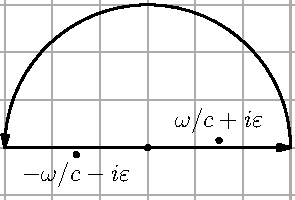
\includegraphics{figuras/contorno.pdf}
    \end{figbox} 
    \vspace{0.1cm}

    Simbólicamente, 
    \begin{equation*}
        \oint = \int_{-\infty}^{\infty} + \cancelto{\scriptstyle0}{\int_{\text{arco}}} = 2\pi i\lim_{\varepsilon\rightarrow0}\text{Res}(\pm\omega/c+i\varepsilon) = \pi i e^{\pm i\omega/c|\mathbf{r}-\mathbf{r}'|},
    \end{equation*}
    por lo que
    \begin{equation}
        \mathcal{G}_\pm(\mathbf{r},\mathbf{r}',\omega) = -\frac{e^{\pm i\omega/c|\mathbf{r}-\mathbf{r}'|}}{4\pi|\mathbf{r}-\mathbf{r}'|}.
    \end{equation}
    Estas funciones sí son de Green de las que nos gustan. Se puede comprobar que cumplen la \cref{eq.1-green_helmholtz_escalar}, aunque ver que realmente sale \(\delta(\mathbf{r}-\mathbf{r}')\) a la derecha requiere pensar un poco en distribuciones. El nombre que se da a estas soluciones viene del tipo de onda que representan cuando devolvemos la evolución temporal \(e^{-i\omega t}\). La solución \(\mathcal{G}_+\) da una onda que sale desde la fuente en \(\mathbf{r}'\) hacia el infinito (onda saliente), mientras que \(\mathcal{G}_-\) está asociada a una onda que converge en \(\mathbf{r}'\) desde el infinito (onda entrante). 
    
    Podemos, además, combinar las soluciones para construir otras nuevas:
    \begin{equation}
        \mathcal{G}_a = \frac{(1+a)\mathcal{G}_+ + (1-a)\mathcal{G}_-}{2}
    \end{equation}
    es claramente solución de la \cref{eq.1-green_helmholtz_escalar} \(\forall a\). Particularmente interesante es la solución con \(a = 0\): \marginexercise{Otra forma de llegar a este resultado es calcular el ``valor principal'' de la integral en la \cref{eq.1-helmholtz_fourier_green}. Hazlo.}  \rnote{Valor princial}{Dada una integral \(\text{I} = \int_\mathbb{R}\mathrm{d}x\, \frac{f(x)}{x-a},\) el valor principal \(P.V.\, \text{I}\) se define como 
    \begin{align*}
        \lim_{\varepsilon\rightarrow 0}&\left[\int_{-\infty}^{a-\varepsilon}\mathrm{d}x \, \frac{f(x)}{x-a}\right.\\
        + &\left.\int_{a+\varepsilon}^\infty\mathrm{d}x\,  \frac{f(x)}{x-a}\right]
    \end{align*} }
    \begin{equation*}
        \mathcal{G}_0(\mathbf{r}, \mathbf{r}', \omega) = \frac{-\cos(\omega/c|\mathbf{r} - \mathbf{r}'|)}{4\pi |\mathbf{r} - \mathbf{r}'|},
    \end{equation*}
    cuya interpretación es de onda estacionaria.

    Veamos los otros dos casos. Si dejamos fuera ambos polos, el resultado es \(\tilde{\mathcal{G}} = 0\), que no tiene ninguna gracia, y no es una función de Green del problema. Por otro lado, si incluimos ambos polos, el resultado
    \begin{equation*}
        \tilde{\mathcal{G}}(\mathbf{r}, \mathbf{r}', \omega) = \frac{-2 \cos(\omega/c|\mathbf{r} - \mathbf{r}'|)}{4\pi |\mathbf{r} - \mathbf{r}'|} = 2\mathcal{G}_0(\mathbf{r}, \mathbf{r}', \omega)
    \end{equation*}
    tampoco es una función de Green, pero casi. Lo fastidia el factor 2.

    De este modo, hemos encontrado dos soluciones básicas (onda saliente y entrante) a la ecuación de Helmholtz escalar y, por linealidad, cualquier combinación de las mismas que preserve la normalización de la \(\delta\) es, también, una función de Green. Hemos dicho al principio de esta discusión que las soluciones son equivalentes. Cualquier onda que podamos escribir con \(\mathcal{G}_+\) puede también escribirse con \(\mathcal{G}_-\). Ahora toca ver por qué.

    Resulta que 
    \begin{equation}
        \mathcal{G}_- - \mathcal{G}_+ = 2i\frac{\sin(\omega/c|\mathbf{r}-\mathbf{r}'|)}{4\pi|\mathbf{r}-\mathbf{r}'|} =: \mathcal{F}(\mathbf{r}, \mathbf{r}', \omega).
    \end{equation}
    Por construcción, \(\mathbf{F}\) es solución de la ecuación de Helmholtz homogénea (sin fuentes). En general, de hecho, podemos imaginar otras soluciones de la ecuación homogénea \(\mathcal{F}'\) y usarlas para construir nuevas funciones de Green a partir de \(\mathcal{G}' = \mathcal{G}_+ + \mathcal{F}'\). La solución construida usando cualquiera de estas funciones de Green se puede obtener con cualquier otra función, siempre y cuando añadamos la contribución homogénea adecuada. Estas soluciones inhomogéneas vendrán, como es lógico, de resolver
    \begin{equation*}
        \nabla^2u^{(+)}_\mathrm{h}(\mathbf{r}, \omega) = - \frac{\omega^2}{c^2}u^{(+)}_\mathrm{h}(\mathbf{r}, \omega),
    \end{equation*}
    y tendremos
    \begin{equation*}
        u^{(+)}(\mathbf{r}, \omega) = u^{(+)}_{\mathrm{h},\pm}(\mathbf{r}, \omega) + \int_{\mathbb{R}^3}\mathrm{d}^3r'\, \mathcal{G}_\pm (\mathbf{r}, \mathbf{r}', \omega) h^{(+)}(\mathbf{r'},\omega),
    \end{equation*}
    donde \(u^{\pm}_\mathrm{h}\) son soluciones inhomogéneas distintas relacionadas por
    \begin{equation*}
        u_{\mathrm{h},+}^{(+)}(\mathbf{r},\omega) = u_{\mathrm{h},-}^{(+)}(\mathbf{r},\omega) + \int_{\mathbb{R}^3}\mathrm{d}^3r'\,\frac{2i\sin(\omega/c|\mathbf{r}-\mathbf{r}'|)}{4\pi|\mathbf{r}-\mathbf{r}'|} h^{(+)}(\mathbf{r}',\omega).
    \end{equation*}

    Dado un problema físico concreto, tendremos que encontrar la solución inhomogénea usando alguna de las funciones de Green, y luego sumar soluciones homogéneas para ajustar la solución total a las condiciones de contorno del problema.\footnote{Según el problema, será más ventajoso usar una función de Green u otra, claro.} Esto sucede también con ecuaciones diferenciales básicas, pero la mayor complejidad de este escenario puede hacer que, a veces, se nos olvide hasta nuestro nombre. 

%     further question:
%     ok. I see. two further questions:

% 1st: is the PV one a legitimate greens function? I get half of what I would get by just shifting both poles inside the contour. that means that it would satisfy the same equation, but with delta/2 as source, right?

% 2nd: what if I choose to shift both poles out of the contour? I arrive at 0 for the greens function, don't I? How can we know that this procedure works (other than just plugging back our solution in) if a specific choice yields directly 0? Is that related to solutions of the homogeneous helmholtz equation (no sources)?

%     Green's function is not necessarily unique since the addition of any solution of the homogeneous equation to one Green's function results in another Green's function. Therefore, if the homogeneous equation has nontrivial solutions, multiple Green's functions exist. Certain boundary value or initial value problems involve finding a Green's function that is nonvanishing only for 
% s
% ≤
% x
% {\displaystyle s\leq x}; in this case, the solution is sometimes called a retarded Green's function.[6] Similarly, a Green's function that is nonvanishing only for 
% s
% ≥
% x
% {\displaystyle s\geq x} is called an advanced Green's function.[7] In such cases, any linear combination of the two Green's functions is also a valid Green's function. Both the advanced and retarded Green's functions are called one-sided, while a Green's function that is nonvanishing for all 
% x
% {\displaystyle x} in the domain of definition is called two-sided.[8]

    
    % Esta ecuación, en rigor, no la hemos visto. De todos modos no hay que estrujarse mucho los sesos. No es más que la ecuación de ondas para \(\mathbf{E}^\perp\) de la \cref{eq.1-ondas_Etransversal}, pero limitándonos a que tanto \(\mathbf{E}^\perp\) como \(\mathbf{j}^\perp\) dependan del tiempo de forma armónica,\footnote{No es una limitación real. Podremos extender el resultado al que lleguemos por linealidad usando Fourier.} igual que hicimos en el vacío:
    % \begin{equation}
    %     \mathbf{E}^\perp(\mathbf{r}, t) = \mathbf{E}^{(+),\perp}(\mathbf{r}, \omega)e^{-i\omega t} + \mathrm{c.c.}
    % \end{equation}
    % Así, la ecuación de Helmholtz para \(\mathbf{E}^\perp\) es
    % \begin{equation}
    %    \left[ \nabla^2 + \frac{\omega^2}{c^2}\right]\mathbf{E}^{(+),\perp}(\mathbf{r}, \omega) = -i\mu_0\omega \mathbf{j}^{(+),\perp}(\mathbf{r}, \omega).
    % \end{equation}
\end{example}

\begin{example}
    {Función de Green de la ecuación de ondas escalar
    \label{ej.1-dalambertian_green}    
    }

    Una vez pasado el largo trago, aunque no malo, del ejemplo anterior, la ecuación de ondas es pan comido. Vamos a disfrutar de los frutos de nuestro trabajo. Observemos que la susodicha,
    \begin{equation}
        \left[\nabla^2 - \frac{1}{c^2}\partial_t^2\right]u(\mathbf{r}, t) = h(\mathbf{r}, t),
    \end{equation}
    no es más que la ecuación de Helmholtz de vuelta en el espacio de \(t\). La solución inhomogénea se construirá, entonces, con la transformada temporal inversa. Explícitamente,
    \begin{equation*}
        \left[\nabla^2 - \frac{1}{c^2}\partial_t^2\right]\mathcal{G}(\mathbf{r}, \mathbf{r}', t, t') = \delta(\mathbf{r}-\mathbf{r}')\delta(t-t')
    \end{equation*}
    o, en el espacio de \(\omega\),
    \begin{equation*}
        \left[\nabla^2 + \frac{\omega^2}{c^2}\right]\mathcal{G}(\mathbf{r}, \mathbf{r}', \omega, t') = \delta(\mathbf{r}-\mathbf{r}')\frac{e^{i\omega t'}}{\sqrt{2\pi}}.
    \end{equation*}
    Es decir, \(\mathcal{G}(\mathbf{r}, \mathbf{r}', \omega, t')\) cumple exactamente la misma ecuación que nos trajo de cabeza en el \cref{ej.1-helmholtz_green}, salvo por el factor que viene de la \(\delta(t-t')\). Podemos reciclar la solución sin ningún pudor y deshacer la transformada de Fourier temporal:
    \begin{align}
        \nonumber
        \mathcal{G}_+(\mathbf{r}, \mathbf{r}', t, t') &= \frac{1}{2\pi}\int_{-\infty}^{\infty}\mathrm{d}\omega\, \frac{-e^{i\omega/c|\mathbf{r}-\mathbf{r}'|}}{4\pi|\mathbf{r}-\mathbf{r}'|}e^{-i\omega(t-t')}\\
        \nonumber
        &=\frac{-1}{4\pi|\mathbf{r}-\mathbf{r}'|} \times\frac{1}{2\pi}\int_{-\infty}^{\infty}\mathrm{d}\omega\, \exp\left\{i\omega\left(\frac{|\mathbf{r}-\mathbf{r}'|}{c} - (t-t')\right)\right\}\\
        \label{eq.1-green_ondas_escalar_retardada}
        &=\frac{-\delta\left((t-t') - \frac{|\mathbf{r}-\mathbf{r}'|}{c} \right)}{4\pi|\mathbf{r}-\mathbf{r}'|}.
    \end{align}
    
    El resultado de la \cref{eq.1-green_ondas_escalar_retardada} es muy interesante. Lo más impresionante es que contiene explícitamente el retardo debido a la propagación de señales con velocidad finita. Nos dice que una perturbación localizada en \(\mathbf{r}'\) en un instante \(t'\) se transmite radialmente y con velocidad \(c\). Además, se deduce de los signos del argumento de la \(\delta\) que \(t>t'\). Por todo esto, esta \(\mathcal{G}_+\) se conoce como función de Green \emph{retardada}.

    Si hubiéramos utilizado \(\mathcal{G}_-\) del ejemplo anterior, habríamos llegado a
        \begin{equation}
        \label{eq.1-green_ondas_escalar_avanzada}
        \mathcal{G}_+(\mathbf{r}, \mathbf{r}', t, t') =\frac{-\delta\left((t-t') + \frac{|\mathbf{r}-\mathbf{r}'|}{c} \right)}{4\pi|\mathbf{r}-\mathbf{r}'|}.
    \end{equation}
    Es igual, salvo por el signo, que implica que \(t<t'\). Por ello, \(\mathcal{G}_-\) recibe el nombre de \emph{adelantada}. La onda en un momento dado \(t\) depende de la fuente en momentos posteriores. Desde el punto de vista de la física, la solución retardada es la que refleja el principio de causalidad. Aun así, igual que en el ejemplo anterior, tanto \(\mathcal{G}_+\) como \(\mathcal{G}_-\), aderezadas por la solución homogénea adecuada, son capaces de expresar cualquier configuración de la onda.

    Un último aspecto que vale la pena discutir en este ejemplo es que podemos extender trivialmente las funciones de Green retardada y adelantada al caso de una onda vectorial como las que se dan en el campo eléctrico. En efecto, hemos visto que \(\mathbf{E}^\perp\), y por tanto sus componentes cartesianas, obedece la \cref{eq.1-ondas_Etransversal}. Por eso pudimos escribir la solución inhomogénea y retardada en la \cref{eq.1-Etransverse_sol}. Aun así, hay algo que puede incomodar conceptualmente. Las funciones de Green que hemos obtenido para la ecuación de ondas no saben nada sobre campos transversales. Sin embargo, \(\mathbf{E}^\perp\) está restringido al subespacio de campos vectoriales transversales. 
    
    Hay dos maneras de atacar el problema. La primera es asegurarse de que la fuente que se introduce en la ecuación de ondas es, ella misma, un campo vectorial transversal, como en las \cref{eq.1-ondas_Etransversal,eq.1-Etransverse_sol}. Así, la solución de \(\mathbf{E}^\perp\) hereda directamente esa propiedad. La otra opción es buscar la función de Green que corresponde al campo eléctrico total, y luego utilizar \(\boldsymbol{\delta}^{\perp/\parallel}\) para quedarnos con la parte que queramos. Explorar esto es el objeto del siguiente y último ejemplo.
\end{example}


\begin{example}
    {Tensor de Green electromagnético
    \label{ej.1-tensorgreen_vacio}}
    Combinando las \cref{eq.1-faradaycarga,eq.1-amperecarga} llegamos, antes de seleccionar la parte transversal, a
    \begin{equation}
        \left[\nabla\times\nabla\times + \frac{1}{c^2}\partial_t^2\right]\mathbf{E}(\mathbf{r}, t) = - \mu_0\partial_t \mathbf{j}(\mathbf{r}, t).
    \end{equation}
    Como queremos hablar del campo eléctrico total, no podemos simplificar el doble rotacional. En su lugar, vamos a desarrollar la teoría del tensor de Green EM: \(\boldsymbol{\mathcal{G}}\). Nota que lo llamamos tensor ahora porque va a tener estructura matricial (\(\text{matriz}\times\text{vector}=\text{vector}\)). Para que sea más conveniente con lo que vendrá en las siguientes secciones, vamos a trabajar directamente en el espacio de frecuencias:
    \begin{equation*}
        \left[\nabla\times\nabla\times - \frac{\omega^2}{c^2}\right]\mathbf{E}^{(+)}(\mathbf{r}, \omega) = i\mu_0 \omega\mathbf{j}^{(+)}(\mathbf{r}, \omega).
    \end{equation*}
    Así, el tensor de Green que buscamos cumple
    \begin{equation}
        \left[\nabla\times\nabla\times - \frac{\omega^2}{c^2}\mathbf{1}\cdot\right]\boldsymbol{\mathcal{G}}(\mathbf{r}, \mathbf{r}', \omega) = \mathbf{1}\delta(\mathbf{r}-\mathbf{r}').
    \end{equation}
    En el espacio de Fourier:
    \begin{equation*}
        \left[-\mathbf{k}\times\mathbf{k}\times - \frac{\omega^2}{c^2}\mathbf{1}\cdot\right]\boldsymbol{\mathcal{G}}(\mathbf{k}, \mathbf{r}', \omega) = \mathbf{1}\frac{e^{-i\mathbf{k}\cdot\mathbf{r}'}}{(2\pi)^{3/2}}.
    \end{equation*}
    Utilizando la identidad del producto triple vectorial podemos masajear la expresión anterior para obtener
    \begin{equation*}
        \left[\left(k^2 - \frac{\omega^2}{c^2}\right)\mathbf{1} - \mathbf{k}\otimes\mathbf{k}\right]\cdot\boldsymbol{\mathcal{G}}(\mathbf{k}, \mathbf{r}', \omega) = \mathbf{1}\frac{e^{-i\mathbf{k}\cdot\mathbf{r}'}}{(2\pi)^{3/2}}.
    \end{equation*}
    Recordemos que en el espacio de Fourier podemos proyectar sobre el vector \(\hat{\mathbf{k}}\) o sobre el subespacio ortogonal. Definimos los proyectores \(\boldsymbol{\mathcal{P}}^\parallel + \boldsymbol{\mathcal{P}}^\perp = \mathbf{1}\), donde \(\boldsymbol{\mathcal{P}}^\parallel = \hat{\mathbf{k}}\otimes\hat{\mathbf{k}}\).\footnote{Si dudas con esto, revisa la \cref{subsubsec.1-campos_transversales}.} Así, \(\boldsymbol{\mathcal{P}}^\parallel\) y \(\boldsymbol{\mathcal{P}}^\perp\) son, ni más ni menos, las deltas longitudinal y transversal en el espacio recíproco. Armados con los proyectores, seguimos manipulando la ecuación y llegamos a 
    \begin{equation*}
        \left[\left(k^2 - \frac{\omega^2}{c^2}\right)\boldsymbol{\mathcal{P}}^\perp - \frac{\omega^2}{c^2}\boldsymbol{\mathcal{P}}^\parallel\right]\cdot\boldsymbol{\mathcal{G}}(\mathbf{k}, \mathbf{r}', \omega) = \mathbf{1}\frac{e^{-i\mathbf{k}\cdot\mathbf{r}'}}{(2\pi)^{3/2}}.
    \end{equation*}
    Como los proyectores son ortogonales, podemos resolver la última expresión para las componentes transversal y longitudinal de \(\boldsymbol{\mathcal{G}}\) por separado y juntar las soluciones para llegar al resultado final
    \begin{equation}
        \boldsymbol{\mathcal{G}}(\mathbf{k}, \mathbf{r}', \omega) = \left[\frac{1}{(2\pi)^{3/2}}\frac{e^{-i\mathbf{k}\cdot\mathbf{r}'}}{k^2-(\omega/c)^2}\right]\boldsymbol{\mathcal{P}}^\perp 
        - \left[\frac{1}{(2\pi)^{3/2}}\frac{e^{-i\mathbf{k}\cdot\mathbf{r}'}}{(\omega/c)^2}\right]\boldsymbol{\mathcal{P}}^\parallel .
    \end{equation}

    Ahora ``solo'' tenemos que invertir la transformada de Fourier de cada trozo y listo. El trozo longitudinal realmente es trivial, no es más que la \(\boldsymbol{\delta}^\parallel\) con un prefactor \((c/\omega)^2\). La parte transversal es un poco más difícil. Aquí daremos simplemente el resultado, pero antes observemos lo siguiente. El trozo transversal no es más que la función de Green de la ecuación de Helmholtz escalar del \cref{ej.1-helmholtz_green} (salvo por un signo \(-\)), multiplicada por el proyector transversal. Utilizando el teorema de la convolución, podemos\rnote[-2cm]{Teorema de la convolución}{La transformada de Fourier de la convolución de dos funciones es igual al producto de las transformadas de Fourier individuales. Hay distintas convenciones con los factores de \(2\pi\).} escribir la componente transversal como \rnote[2cm]{Convolución}{Dadas dos funciones, \(f\) y \(g\), su convolución es \([f*g](x) = \int_\mathbb{R}\mathrm{d}x'\, f(x')g(x-x')\).} \marginexercise{Toma nuestra definición de la transformada de Fourier y demuestra el teorema de la convolución}
    \begin{equation*}
        \boldsymbol{\mathcal{G}}^\perp(\mathbf{r}, \mathbf{r}', \omega) = - \int_{\mathbb{R}^3}\mathrm{d}\mathbf{r}''\, \mathcal{G}_+(\mathbf{r}, \mathbf{r}'',\omega)\boldsymbol{\delta}^\perp(\mathbf{r}''-\mathbf{r}').
    \end{equation*}
    Esta fórmula cierra el círculo respecto a lo que comentábamos en el último párrafo del ejemplo anterior. La delta se encarga de asegurar que solo la componente transversal de una fuente arbitraria afecte al \(\mathbf{E}^\perp\).
    
    Vamos al resultado completo:
    \begin{align}
        \nonumber
        \boldsymbol{\mathcal{G}}(\mathbf{r}, \mathbf{r}', \omega) &= - \frac{c^2}{3\omega^2}\mathbf{1}\delta(\boldsymbol{\rho}) - \frac{c^2 e^{i\omega \rho/c}}{4\pi\omega^2|\mathbf{r}-\mathbf{r}'|^3}\left\{\left[1-i\frac{\omega\rho}{c}-\left(\frac{\omega\rho}{c}\right)^2\right]\mathbf{1}\right.\\
        &\phantom{=}-\left.\left[3-3i\frac{\omega\rho}{c} - \left(\frac{\omega\rho}{c}\right)^2\right]\hat{\boldsymbol{\rho}}\otimes\hat{\boldsymbol{\rho}}\right\},
    \end{align}
    donde \(\boldsymbol{\rho} = \mathbf{r}-\mathbf{r}'\). La fórmula es tirando a fea, pero su interpretación es muy sencilla. Imaginemos un dipolo puntual en \(\mathbf{r}_\mathrm{d}\), dos cargas opuestas infinitesimalmente juntas, cuyo momento dipolar \(\mathbf{d}\) oscila en el tiempo con frecuencia \(\omega\). La corriente asociada a dicho dipolo es \(\mathbf{j}^{(+)}(\mathbf{r}, \omega) = -i\omega\mathbf{d} \delta(\mathbf{r}-\mathbf{r}_\mathrm{d})\). De este modo, el campo eléctrico asociado al dipolo es \marginexercise{Comprueba que, en el límite estático (\(\omega\rightarrow0\)), se recupera el campo electrostático de un dipolo.}
    \begin{equation*}
        \mathbf{E}^{+}(\mathbf{r}, \omega) = \frac{\omega^2}{c^2}\boldsymbol{\mathcal{G}}(\mathbf{r}, \mathbf{r}_\mathrm{d}, \omega)\cdot\mathbf{d}.
    \end{equation*}
    En otras palabras, \(\boldsymbol{\mathcal{G}}\) nos dice qué efecto tiene en cada punto del espacio una perturbación eléctrica localizada. Conocer el tensor de Green es equivalente a conocer la distribución del campo eléctrico en el espacio dado un dipolo puntual.
    
\end{example}
Un último apunte sobre nomenclatura. Al tensor de Green del \cref{ej.1-tensorgreen_vacio} se lo conoce como tensor de Green del vacío, a pesar de que ya hemos introducido las cargas. El motivo es que nos dice cómo se propaga el campo EM entre esas cargas, a través del espacio vacío. Pero el campo EM siempre se propaga así, ¿por qué especificar ``del vacío''? El asunto es cuando hay materiales de por medio la propagación del campo se ve alterada; tenemos reflexión, refracción y difracción. Existirá, por tanto, un tensor de Green modificado que dé cuenta de todo ello. Por supuesto, fundamentalmente esos materiales están formados por partículas cargadas, así que todo lo que hemos hecho hasta ahora sigue siendo válido. Lo que pasa es que cuando son tantísimas partículas es más práctico pasar a una descripción continua de la materia, cuya respuesta ante campos EM se codifica en \(\varepsilon\) y \(\mu\), la permitividad y permeabilidad relativas. Estas propiedades modifican la ecuación de ondas, que a su vez da lugar al tensor de Green modificado. El inicio de la \cref{sec.2-medioslineales} está dedicado precisamente a esto.

\subsubsection{Perspectiva lagrangiana y hamiltoniana de nuevo} 
\label{subsubseq.1-lagrangecargas}

Igual que en el vacío, las ecuaciones de la electrodinámica en presencia de cargas [\cref{eq.1-gaussEcarga,eq.1-gaussBcarga,eq.1-amperecarga,eq.1-faradaycarga,eq.1-newton_lorentz}] se pueden obtener como ecuaciones de movimiento de un lagrangiano o hamiltoniano. El lagrangiano genérico es \marginexercise[-0.95cm]{Demuestra que una transformación gauge en el lagrangiano únicamente añade un término de la forma \(\nabla\cdot(\mathbf{j}\chi) + \partial_t(\rho\chi)\). ¿Qué efecto tiene un término así en las ecuaciones de movimiento? ¿Qué papel juega la conservación de la carga?}
\begin{align}
    \nonumber
    L &= \sum_\alpha \frac{m_\alpha}{2}\dot{\mathbf{r}}_\alpha^2(t) + \frac{\varepsilon_0}{2} \int_{\mathbb{R}^3}\mathrm{d}^3r\, \left[\mathbf{E}^2(\mathbf{r}, t) - c^2\mathbf{B}^2(\mathbf{r})\right] \\
    &\phantom{=} + \int_{\mathbb{R}^3}\mathrm{d}^3r\, \big[\mathbf{j}(\mathbf{r})\cdot\mathbf{A}(\mathbf{r}, t) - \mathbf{\rho}(\mathbf{r}, t)\phi(\mathbf{r}, t)\big] .
\end{align}
El primer término es la energía cinética de las partículas. Luego tenemos el lagrangiano del campo y, finalmente, la interacción que se conoce como ``acoplamiento mínimo''. 

A diferencia del vacío, en presencia de cargas el campo eléctrico tiene componente longitudinal, de modo que el primer término del lagrangiano del campo se descompone en
\begin{equation*}
    \frac{\varepsilon_0}{2}\int_{\mathbb{R}^3}\mathrm{d}^3r\,\left\{\left[\mathbf{E}^\parallel(\mathbf{r}, t)\right]^2 + \left[\mathbf{E}^\perp(\mathbf{r}, t)\right]^2\right\}.
\end{equation*}
De estos dos trozos, el primero puede escribirse como \marginexercise[0.5cm]{Demuestra esta relación. Para ello, comprueba que el potencial escalar de Coulomb de una distribución \(\rho\) cumple \(\nabla\phi_\mathrm{C} = -\mathbf{E}^\parallel\), usa integración por partes, recuerda la ecuación de Poisson: \(\nabla^2\phi_\mathrm{C} = -\rho\), y descarta la autoenergía de Coulomb (sumandos con \(\alpha=\beta\)).}
\begin{align*}
    \frac{\varepsilon_0}{2}\int_{\mathbb{R}^3}\mathrm{d}^3r\, \left[\mathbf{E}^\parallel(\mathbf{r}, t)\right]^2 &= \frac{1}{2}\int\mathrm{d}^3r\, \rho(\mathbf{r}, t)\phi_\mathrm{C}(\mathbf{r}, t) = \frac{1}{8\pi\varepsilon_0}\int_{\mathbb{R}^3}\mathrm{d}^3r\,\mathrm{d}^3r'\,\frac{\rho(\mathbf{r}, t)\rho(\mathbf{r'}, t)}{\left|\mathbf{r}-\mathbf{r}'\right|}\\
    & = \sum_{\alpha\neq\beta} \frac{1}{8\pi\varepsilon_0} \frac{q_\alpha q_\beta}{\left|\mathbf{r}_\alpha(t) - \mathbf{r}_\beta(t)\right|},
\end{align*}
donde \(\phi_\mathrm{C}\) es el potencial de Coulomb:
\begin{equation}
    \phi_\mathrm{C}(\mathbf{r}, t) = \frac{1}{4\pi\varepsilon_0}\int\mathrm{d}^3\mathbf{r}'\, \frac{\rho(\mathbf{r}', t)}{|\mathbf{r}-\mathbf{r}'|} = \sum_\alpha\frac{1}{4\pi\varepsilon_0}\frac{q_\alpha}{|\mathbf{r}-\mathbf{r}_\alpha(t)|}.
\end{equation}
Es importante observar que, aunque hemos escrito \(\phi_\mathrm{C}\) en un paso intermedio, no hemos fijado el gauge en ningún momento. En cierto modo, \(\phi_\mathrm{C}\) no es más que una función de las cargas conveniente hasta este punto. A nivel del lagrangiano lo que aparece como variable es \(\phi\), no \(\phi_\mathrm{C}\). 

Ahora sí, por sencillez, vamos a fijar el gauge de Coulomb. Para ello, reemplazamos \(\mathbf{A}\) por \(\mathbf{A}_\mathrm{C} =\mathbf{A}^\perp\), y \(\phi\) por \(\phi_\mathrm{C}\). Fijando este gauge, la única coordenada generalizada del campo EM restante es \(\mathbf{A}_\mathrm{C}\). El potencial escalar ha sido ``resuelto'' en términos de \(\mathbf{r}_\alpha\), igual que en el vacío quedó resuelto como \(\phi_\mathrm{C}^{(\text{vacío})} = 0\). En este gauge, el lagrangiano se reduce a \marginexercise{Completa los pasos que faltan.}
\begin{align}
    L &= \sum_\alpha \frac{m_\alpha}{2}\dot{\mathbf{r}}_\alpha^2(t) - \sum_{\alpha\neq\beta} \frac{1}{8\pi\varepsilon_0} \frac{q_\alpha q_\beta}{\left|\mathbf{r}_\alpha(t) - \mathbf{r}_\beta(t)\right|} \\
    \nonumber
    &\phantom{=} + \int_{\mathbb{R}^3}\mathrm{d}^3r\, \left\{\frac{\varepsilon_0}{2}\left[\left(\dot{\mathbf{A}}_\mathrm{C}(\mathbf{r}, t)\right)^2 - c^2\left(\nabla\times \mathbf{A}_\mathrm{C}(\mathbf{r}, t)\right)^2\right] + \mathbf{j}(\mathbf{r}, t)\cdot\mathbf{A}_\mathrm{C}(\mathbf{r}, t) \right\}.
\end{align}

Para calcular el hamiltoniano, obtenemos primero los momentos canónicos\marginexercise{Completa los pasos de forma explícita.}
\begin{subequations}
    \begin{align}
        \mathbf{p}_\alpha(t) &= \frac{\partial L}{\partial \mathbf{r}_\alpha} = m_\alpha\dot{\mathbf{r}}_\alpha(t) + q_\alpha \mathbf{A}_\mathrm{C}(\mathbf{r}_\alpha(t), t),\text{ y}\\
        \boldsymbol{\Pi}(\mathbf{r}, t) &= \frac{\delta L}{\delta \partial_t(\mathbf{A}_\mathrm{C})} = \varepsilon_0 \dot{\mathbf{A}}_\mathrm{C}(\mathbf{r}, t) = -\varepsilon_0 \mathbf{E}^\perp(\mathbf{r}, t).
    \end{align}
\end{subequations}
Un detalle que puede pasar inadvertido es que el momento canónico de las cargas \emph{no coincide} con el momento cinético \(m_\alpha \dot{\mathbf{r}}_\alpha\). Está desplazado por un factor \(q_\alpha\mathbf{A}_\mathrm{C}(\mathbf{r}_\alpha)\). A priori, podríamos haber dicho que el momento de las partículas tendría que ver con las partículas únicamente, pero no es así. El momento canónico de las partículas contiene dentro de sí información del propio campo EM. En este detalle aparentemente insulso se esconden cuestiones interesantes sobre cómo escribir la interacción.\footnote{No profundizaremos nada más, pero por concretar un poco, diremos lo siguiente. El momento de las cargas está desplazado, mientras que el del campo sigue igual siendo el mismo que en el vacío. Resulta que es posible hacer una transformación canónica que desplaza los momentos de manera que \(\mathbf{p}_\alpha^\prime\) coincide (casi) con el cinético, mientras que \(\boldsymbol{\Pi}\) pasa a ser \(-\varepsilon_0 \mathbf{E}^\perp - \mathbf{P}^\perp\), donde \(\mathbf{P}\) es la densidad de polarización de la materia. Así se llega al llamado hamiltoniano multipolar, equivalente al de acoplamiento mínimo.} Finalmente, el hamiltoniano de acoplamiento mínimo en el gauge de Coulomb es
\begin{align}
    H &= \sum_\alpha \frac{\big[\mathbf{p}_\alpha(t) - q_\alpha \mathbf{A}_\mathrm{C}(\mathbf{r}_\alpha(t), t)\big]^2}{2m_\alpha} + \sum_{\alpha\neq\beta} \frac{1}{8\pi\varepsilon_0} \frac{q_\alpha q_\beta}{\left|\mathbf{r}_\alpha(t) - \mathbf{r}_\beta(t)\right|} \\
    \nonumber
    &\phantom{=} + \frac{\varepsilon_0}{2} \int_{\mathbb{R}^3}\mathrm{d}^3r\, \left[\left(\mathbf{E}^\perp(\mathbf{r}, t)\right)^2 - c^2\left(\mathbf{B}(\mathbf{r}, t)\right)^2\right] .
\end{align}



 
% \subsection{Formulación covariante}
% \label{subsec.1-formulacion_covariante}

% Las leyes de Maxwell tienen la propiedad de ser invariantes bajo transformaciones de Lorentz; la electrodinámica es una teoría intrínsecamente relativista o covariante. Desde un punto de vista fundamental es tremendamente importante. No obstante, la relevancia práctica de este hecho en el ámbito de la fotónica es ciertamente reducida. Aun así, vamos a dedicar esta sección a exponer y destacar las ecuaciones de la electrodinámica. 


% Recurso interesante: \href{https://webhome.phy.duke.edu/~rgb/Class/phy319/phy319/node120.html}{notas de Robert G. Brown (Universidad de Duke)}.

% blablabla
%     la formulación lagrangiana de la electrodinámica como teoría clásica de campos. En primer lugar, debemos identificar las coordenadas y velocidades generalizadas, y construir con ellas un lagrangiano cuyas ecuaciones de movimiento sean las de Maxwell.
    
%     -- lagrangiano del campo libre
    
%     -- derivación de las ecuaciones de Maxwell en el vacío
    

